% !TEX root = Tesi.tex
\chead{}
\chapter{Our approach to modeling}

While in the last chapter we introduced three different streams of real usage data obtained both from the physical and the virtual world, we now focus on expanding those representations in a more detailed way with the help of the Model-Driven Engineering techniques briefly described in \ref{model-driven-techniques}. 
Concretely, the goal of the first two sections is to illustrate the defining languages (metamodels) for both the real usage data and the eCommerce platform interactions described in the previous examples. Besides, we will generate actual models based upon those metamodels, which represent the very same information.
Finally, in the last section, we will use the same model generation for updating the models instantiated previously, leveraging model transformation techniques based upon usage pattern detection resulting from the Big Data analysis.

\section{Real usage data modeling}

\subsection{Metamodel}

The representation of the real usage data starts from the definition of the metamodel that defines the languages and processes from which to form a model without making statements about its content. In fact, a metamodel is itself a model that is used to describe another model by using a modeling language at a different level of abstraction.  

Figure in \ref{fig:real-usage-data-metamodel-diagram} describes the processed metamodel as a UML Class Diagram according to the data retrieved for our real usage data analysis.

\vspace{0.5cm}
\begin{figure}[H]
  \centering
    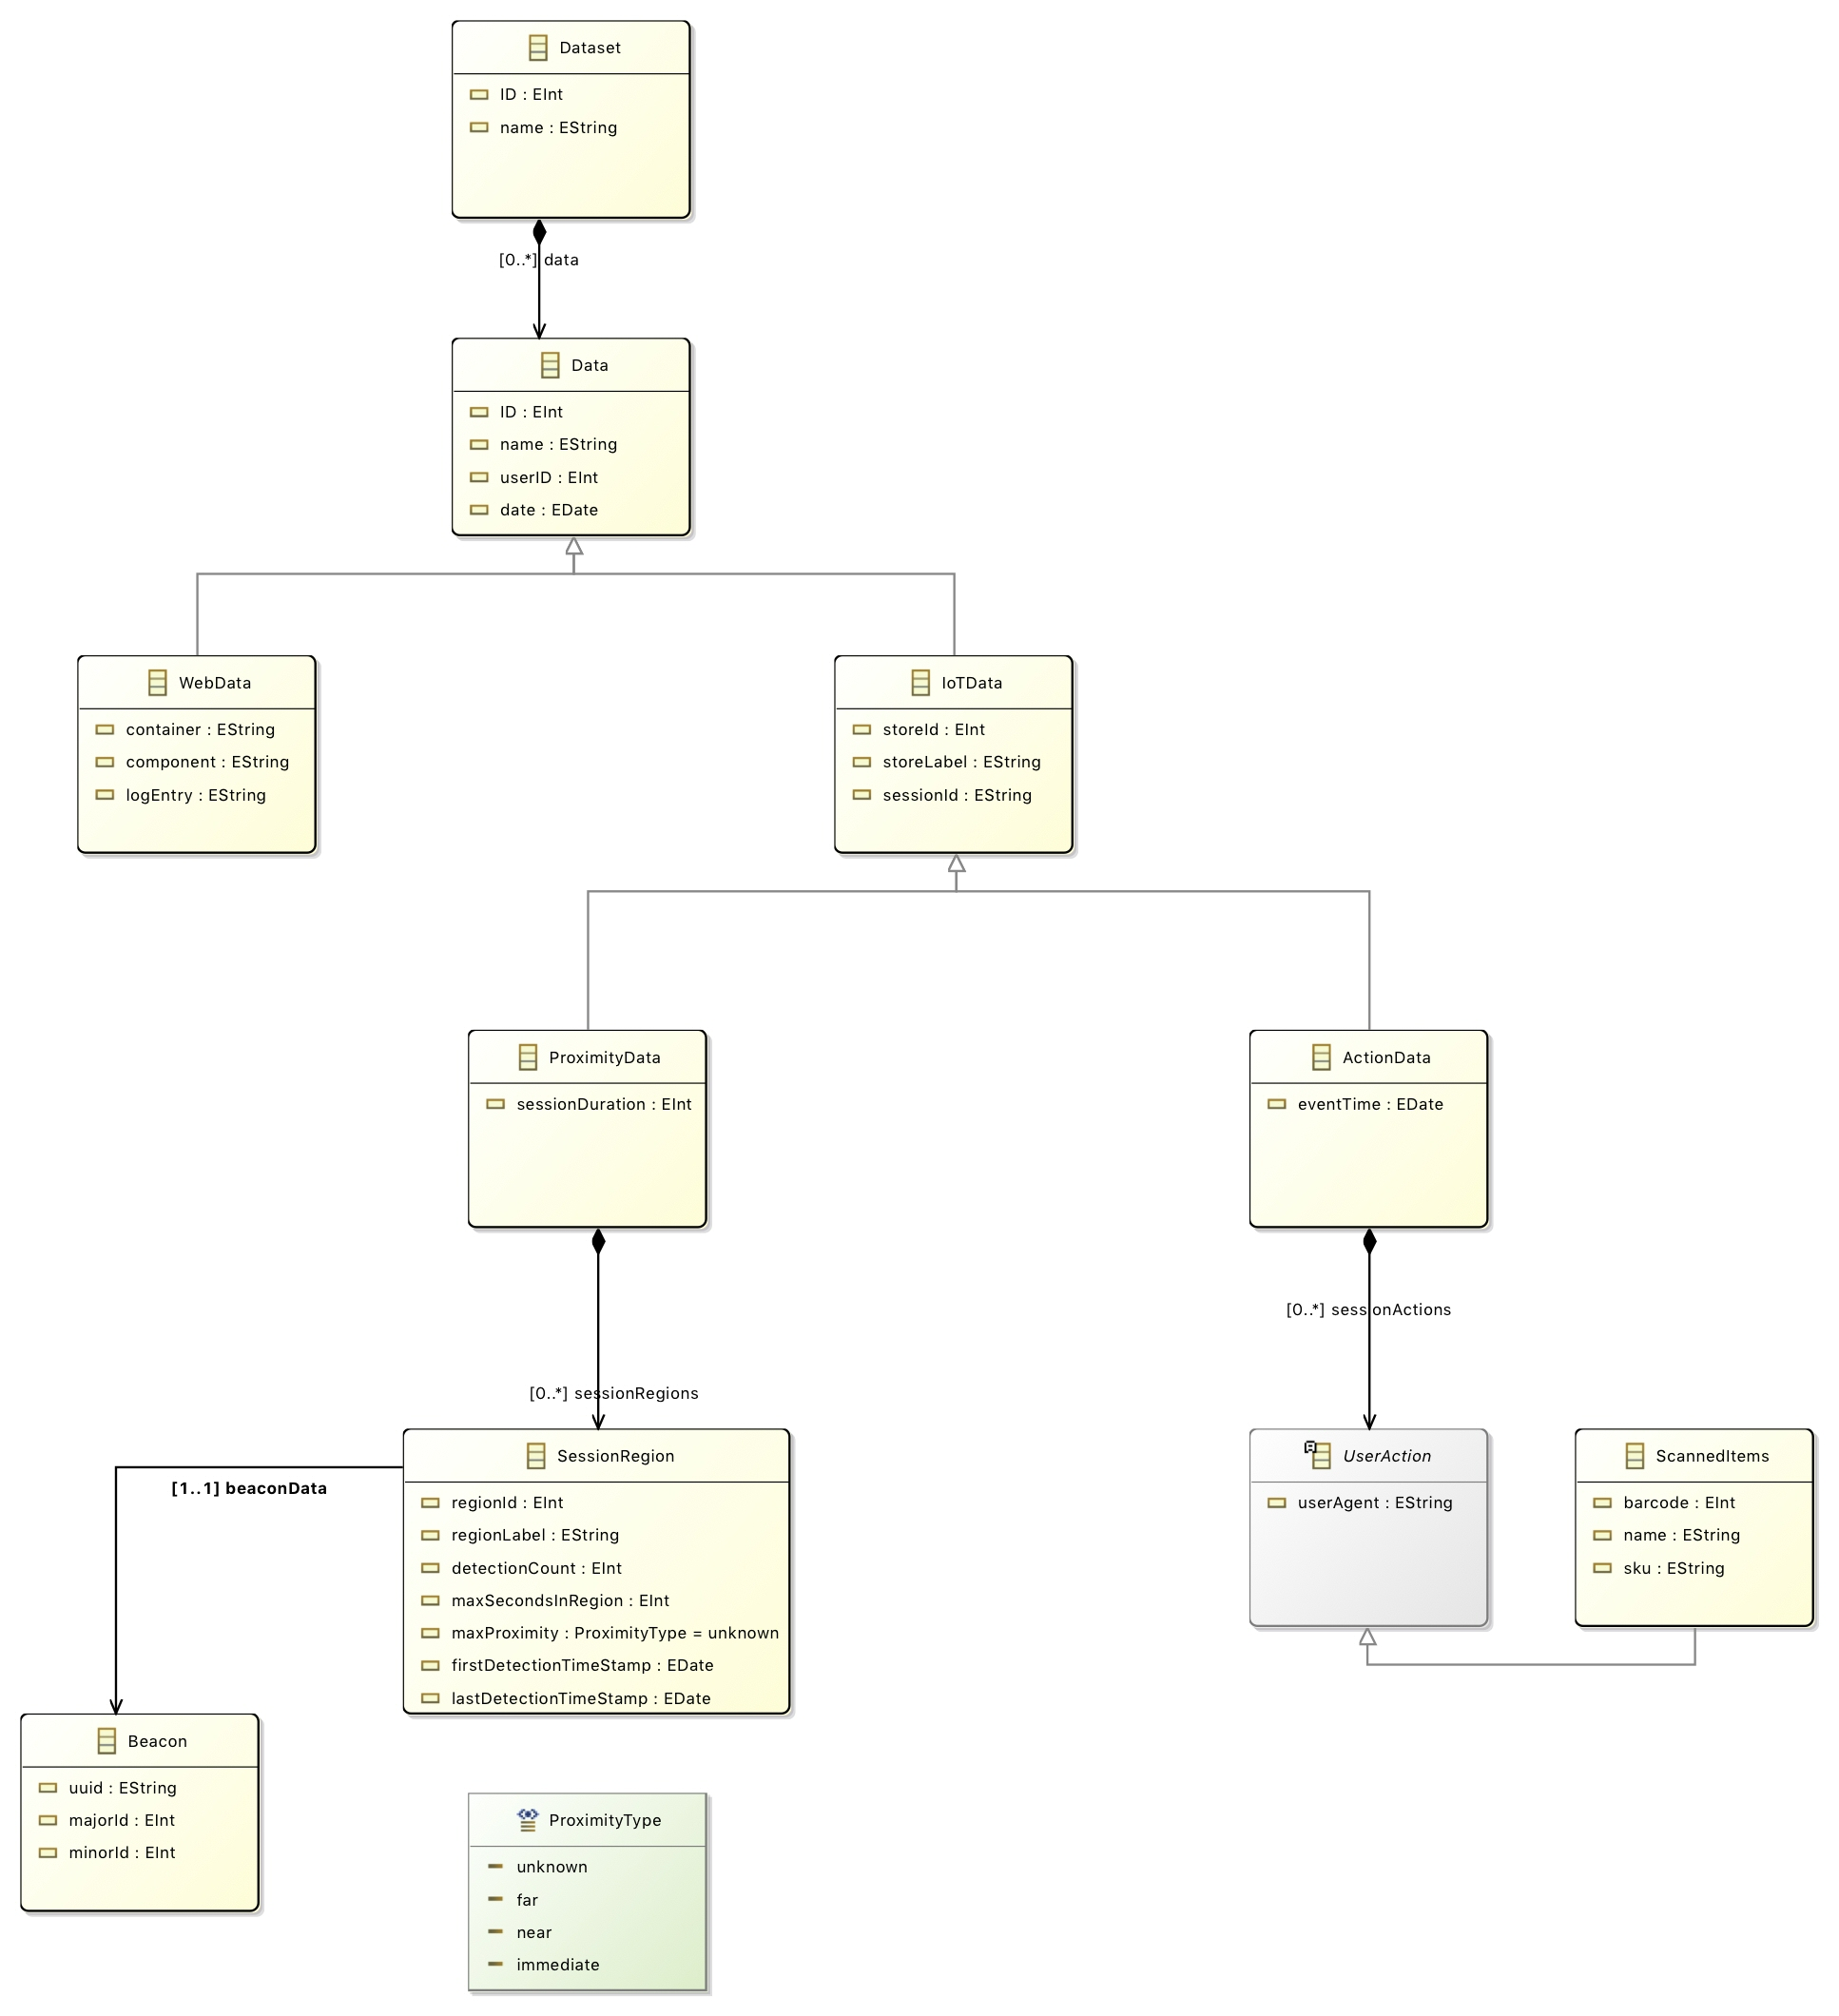
\includegraphics[height=19cm]{images/diagrams/RealUsageDataMetamodel.jpg}
  \caption{Real Usage Data Metamodel Diagram Class}
  \label{fig:real-usage-data-metamodel-diagram}
\end{figure}
\vspace{0.5cm}

\newpage
\subsection{Model}
\label{real-usage-data-model}

The RealUsageData metamodel defined above allows us to create dynamic instances that precisely map the real usage data collected both from web mining process and from IoT devices tracking. Figure \ref{fig:real-usage-data-model} illustrates this processed model in its ecore representation form in Eclipse Modeling Tools (EMF). The figure is followed by the corresponding model content.

\vspace{0.5cm}
\begin{figure}[H]
  \centering
    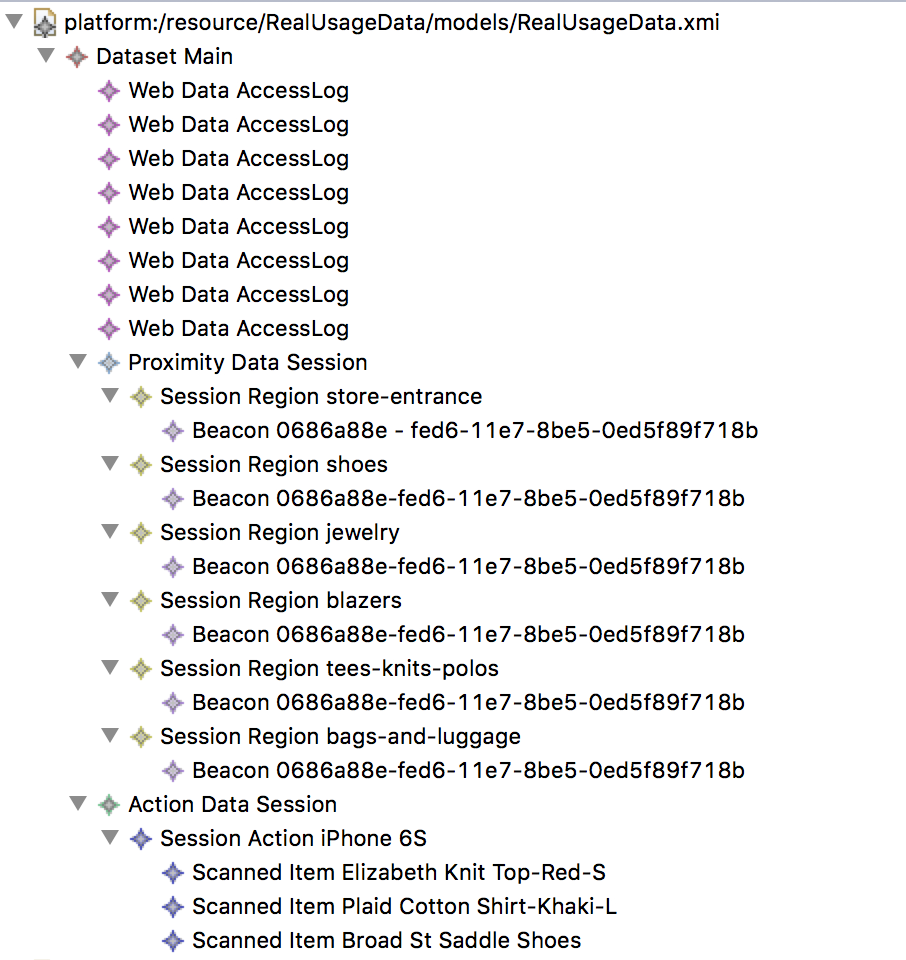
\includegraphics[height=12cm]{images/diagrams/RealUsageDataModel.png}
  \caption{Real Usage Data Model in EMF}
  \label{fig:real-usage-data-model}
\end{figure}
\vspace{0.5cm}

\lstset{language=XML}
\begin{lstlisting} 
<?xml version="1.0" encoding="UTF-8"?>
<RealUsageData:Dataset
    xmi:version="2.0"
    xmlns:xmi="http://www.omg.org/XMI"
    xmlns:xsi="http://www.w3.org/2001/XMLSchema-instance"
    xmlns:RealUsageData="RealUsageData"
    xsi:schemaLocation="RealUsageData ../metamodels/RealUsageData.ecore"
    ID="1" name="Main">
  <data xsi:type="RealUsageData:WebData"
      ID="1"
      name="AccessLog"
      userID="3045678"
      date="2017-11-29T17:06:49.000+0100"
      viewContainer="Homepage"
      viewComponent="TopMenu"
      eventType="click"
      parameterBindingGroup="Category/5"
      logEntry="GET /men.html / 200 0 - 29505"/>
  <data xsi:type="RealUsageData:WebData"
      ID="2"
      name="AccessLog"
      userID="3045678"
      date="2017-11-29T17:07:04.000+0100"
      viewContainer="Category #5"
      viewComponent="CategoryList"
      eventType="click"
      parameterBindingGroup="Category/15"
      logEntry="GET /men/shirts.html 200 0 - 29505"/>
  <data xsi:type="RealUsageData:WebData"
      ID="3"
      name="AccessLog"
      userID="3045678"
      date="2017-11-29T07:08:40.000+0100"
      viewContainer="Category #15"
      viewComponent="ProductList"
      eventType="click"
      parameterBindingGroup="Product/404"
      logEntry="GET /men/shirts/plaid-cotton-shirt-476.html 200 0 - 29505"/>
  <data xsi:type="RealUsageData:WebData"
      ID="4"
      name="AccessLog"
      userID="3045678"
      date="2017-12-04T06:37:15.000+0100"
      viewContainer="Product #404"
      viewComponent="RelatedProductList"
      eventType="click"
      parameterBindingGroup="Product/413"
      logEntry="GET /core-striped-sport-shirt-551.html 200 0 - 29505"/>
  <data xsi:type="RealUsageData:WebData"
      ID="5"
      name="AccessLog"
      userID="3045678"
      date="2017-12-04T06:37:21.000+0100"
      viewContainer=""
      viewComponent=""
      eventType="backButton"
      parameterBindingGroup=""
      logEntry="GET /men/shirts/plaid-cotton-shirt-476.html 200 0 - 29505"/>
  <data xsi:type="RealUsageData:WebData"
      ID="6"
      name="AccessLog"
      userID="3045678"
      date="2017-12-04T06:38:06.000+0100"
      viewContainer="Product #404"
      viewComponent="TopMenu"
      eventType="click"
      parameterBindingGroup="Category/16"
      logEntry="GET /men/tees-knits-and-polos.html 200 0 - 29505"/>
  <data xsi:type="RealUsageData:WebData"
      ID="7"
      name="AccessLog"
      userID="3045678"
      date="2017-12-04T06:38:20.000+0100"
      viewContainer="Category #16"
      viewComponent="TopSearch"
      eventType="submit"
      parameterBindingGroup="SearchText/blazer"
      logEntry="GET /catalogsearch/result/?q=blazer 200 0 - 29505"/>
  <data xsi:type="RealUsageData:WebData"
      ID="8"
      name="AccessLog"
      userID="3045678"
      date="2017-12-04T06:38:20.000+0100"
      viewContainer="Search Results"
      viewComponent="ProductList"
      eventType="click"
      parameterBindingGroup="Product/407"
      logEntry="GET /stretch-cotton-blazer-587.html 200 0 - 29505"/>
  <data xsi:type="RealUsageData:ProximityData"
      ID="9"
      name="Session"
      userID="3045678"
      date="2018-02-21T18:16:07.000+0100"
      storeId="8784"
      storeLabel="Madison1"
      sessionId="89376f84-065b -11e8- ba89-0ed5f89f718b"
      sessionDuration="345">
    <sessionRegions
        regionId="156"
        regionLabel="store-entrance"
        detectionCount="2"
        maxSecondsInRegion="5"
        firstDetectionTimeStamp="2018-02-21T18:09:07.000+0100"
        lastDetectionTimeStamp="2018-02-21T18:16:02.000+0100">
      <beaconData
          uuid="0686a88e - fed6-11e7-8be5-0ed5f89f718b"
          majorId="2553"
          minorId="79"/>
    </sessionRegions>
    <sessionRegions
        regionId="645"
        regionLabel="shoes"
        detectionCount="1"
        maxSecondsInRegion="24"
        maxProximity="near"
        firstDetectionTimeStamp="2018-02-21T18:09:20.000+0100"
        lastDetectionTimeStamp="2018-02-21T18:09:20.000+0100">
      <beaconData
          uuid="0686a88e-fed6-11e7-8be5-0ed5f89f718b"
          majorId="19029"
          minorId="49"/>
    </sessionRegions>
    <sessionRegions
        regionId="6875"
        regionLabel="jewelry"
        detectionCount="1"
        maxSecondsInRegion="15"
        maxProximity="far"
        firstDetectionTimeStamp="2018-02-21T18:10:15.000+0100"
        lastDetectionTimeStamp="2018-02-21T18:10:15.000+0100">
      <beaconData
          uuid="0686a88e-fed6-11e7-8be5-0ed5f89f718b"
          majorId="38415"
          minorId="59"/>
    </sessionRegions>
    <sessionRegions
        regionId="2563"
        regionLabel="blazers"
        detectionCount="1"
        maxSecondsInRegion="195"
        maxProximity="immediate"
        firstDetectionTimeStamp="2018-02-21T18:11:01.000+0100"
        lastDetectionTimeStamp="2018-02-21T18:11:01.000+0100">
      <beaconData
          uuid="0686a88e-fed6-11e7-8be5-0ed5f89f718b"
          majorId="25911"
          minorId="27"/>
    </sessionRegions>
    <sessionRegions
        regionId="456"
        regionLabel="tees-knits-polos"
        detectionCount="1"
        maxSecondsInRegion="10"
        maxProximity="immediate"
        firstDetectionTimeStamp="2018-02-21T18:14:56.000+0100"
        lastDetectionTimeStamp="2018-02-21T18:14:56.000+0100">
      <beaconData
          uuid="0686a88e-fed6-11e7-8be5-0ed5f89f718b"
          majorId="42037"
          minorId="36"/>
    </sessionRegions>
    <sessionRegions
        regionId="998"
        regionLabel="bags-and-luggage"
        detectionCount="1"
        maxSecondsInRegion="7"
        maxProximity="far"
        firstDetectionTimeStamp="2018-02-21T18:15:12.000+0100"
        lastDetectionTimeStamp="2018-02-21T18:15:12.000+0100">
      <beaconData
          uuid="0686a88e-fed6-11e7-8be5-0ed5f89f718b"
          majorId="37931"
          minorId="85"/>
    </sessionRegions>
  </data>
  <data xsi:type="RealUsageData:ActionData"
      ID="10"
      name="Session"
      userID="3045678"
      date="2018-02-22T15:27:09.000+0100"
      storeId="8784"
      storeLabel="Madison1"
      sessionId="89376f84-065b-11e8-ba89-0ed5f89f718b"
      sessionDuration="456">
    <sessionActions
        userAgent="iPhone 6S">
      <scannedItems
          barcode="042100005264"
          name="Elizabeth Knit Top-Red-S"
          sku="wbk012c-Red-S"/>
      <scannedItems
          barcode="042100005931"
          name="Plaid Cotton Shirt-Khaki-L"
          sku="msj006c-Khaki-L"/>
      <scannedItems
          barcode="042100007717"
          name="Broad St Saddle Shoes"
          sku="shm00110"/>
    </sessionActions>
  </data>
</RealUsageData:Dataset>
\end{lstlisting}
\vspace{0.5cm}
\section{eCommerce application modeling}

As we have briefly introduced in \ref{the-ifml-language}, IFML is used to design platform independent-level models that can be used to define the interactions between the users of an application and the application itself. At its core, IFML is meant to be flexible and straightforward, but perhaps more importantly, the language is intended to be abstract enough to allow the definition of the main traits of an application front-end making as few visual commitments as possible. Furthermore, its extendibility  allows modelers and designers to specialise specific components, enriching the semantics of their models and making the diagrams more readable.

In fact, the models generated using IFML describe the user-interface components required at the front-end of the application, without specifying layout details of these elements. Such approach enhances the separation of concerns among developers and UX designers, in which the latter builds the user interface according to an interaction flow model. Besides defining components of the User Interface, these models explain how data flows among different sections of the application upon triggering events, and introduces the business logic carried out using that data.

\subsection{IFML Metamodel}

The IFML metamodel is organised into three packages: the Core, the Extension, and the DataTypes. The Core package contains the concepts that build up the interaction infrastructure of the language concerning InteractionFlowElements, InteractionFlows and Parameters. The Extension package extends the Core package components with more complex behaviours. The DataTypes package, in its turn, contains the custom data types defined by IFML.

\vspace{0.5cm}
\begin{figure}[H]
  \centering
    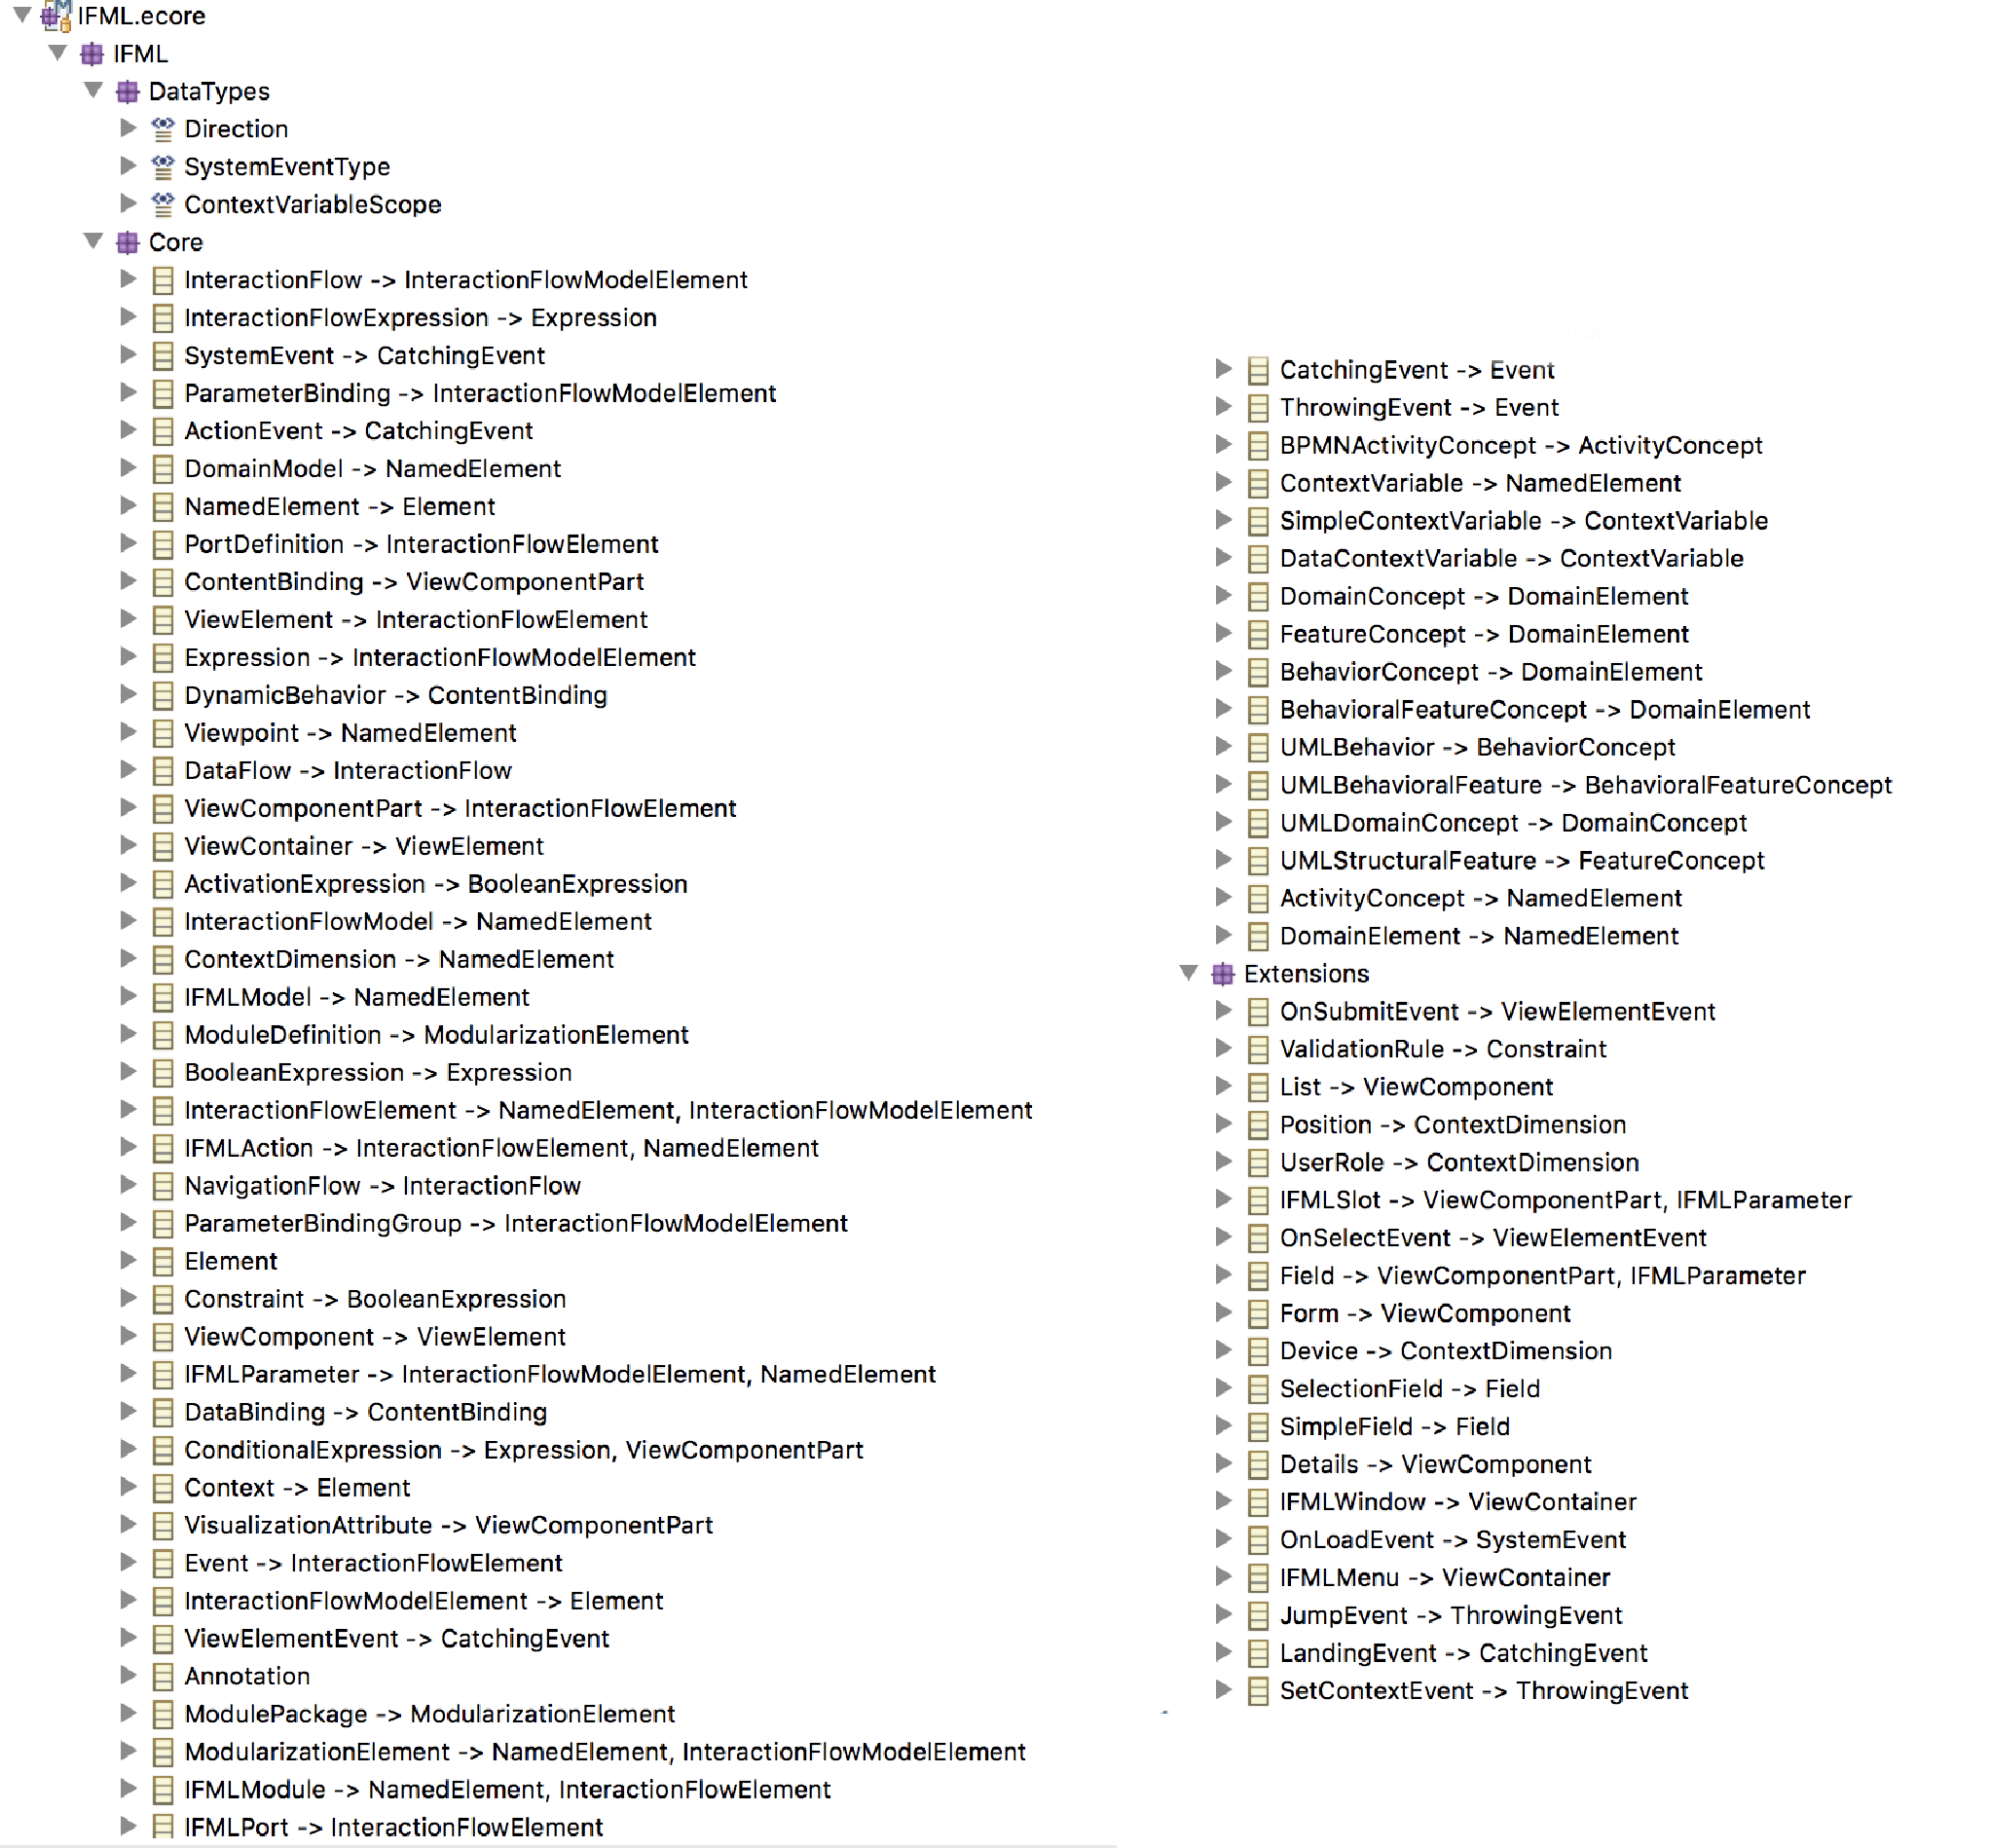
\includegraphics[width=16cm]{images/diagrams/ifml-ecore.png}
  \caption{IFML metamodel in EMF}
  \label{fig:ifml-ecore-representation}
\end{figure}
\vspace{0.5cm}

By using the primitive data types from the UML metamodel and a UML representation for the IFML Domain Model, the IFML metamodel specifies a set of UML metaclasses as the foundation for the IFML metaclasses.

\newpage
The following structure is a high-level representation of the IFML metamodel and its areas of concern:

\begin{itemize}
  \item IFML Model
  \item Interaction Flow Model
  \item Interaction Flow Elements
  \item View Elements
  \item Events
  \item Specific Events and View Components
  \item Parameters
  \item Expressions
  \item ContentBinding
\end{itemize}

Figure \ref{fig:simple-ifml-core-model} shows an excerpt of the IFML metamodel. The \textit{IFMLModel} is the top-level container of all the model elements and represents an \textit{IFMLModel}. It contains an \textit{InteractionFlowModel} that is the user view of an application, a \textit{DomainModel} represented in UML, and optional ViewPoints. The concepts extending \textit{ViewContainer}, \textit{ViewComponents}, \textit{ViewComponentPart}, and \textit{ViewElementEvent} represent the visual elements of an \textit{IFMLModel}.

\vspace{0.5cm}
\begin{figure}[H]
  \centering
    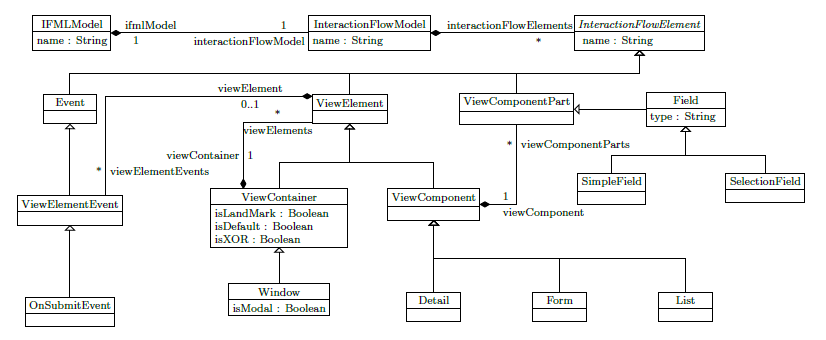
\includegraphics[width=15cm]{images/diagrams/ifml-metamodel.png}
  \caption{Class diagram of an IFML subset.}
  \label{fig:simple-ifml-core-model}
\end{figure}
\vspace{0.5cm}

\subsection{Model}

As mentioned previously, interaction flow models are described using the Interaction Flow Modelling Language and, together with the domain model and optionally viewpoints, they form the core of the \textit{IFMLModel}.

Essentially, the goal of the domain model is to offer to the interaction flow references about the available content. An example of a domain model for an e-commerce website is given in Figure~\ref{fig:domain-model-uml-ecommerce}.

\vspace{0.5cm}
\begin{figure}[H]
  \centering
    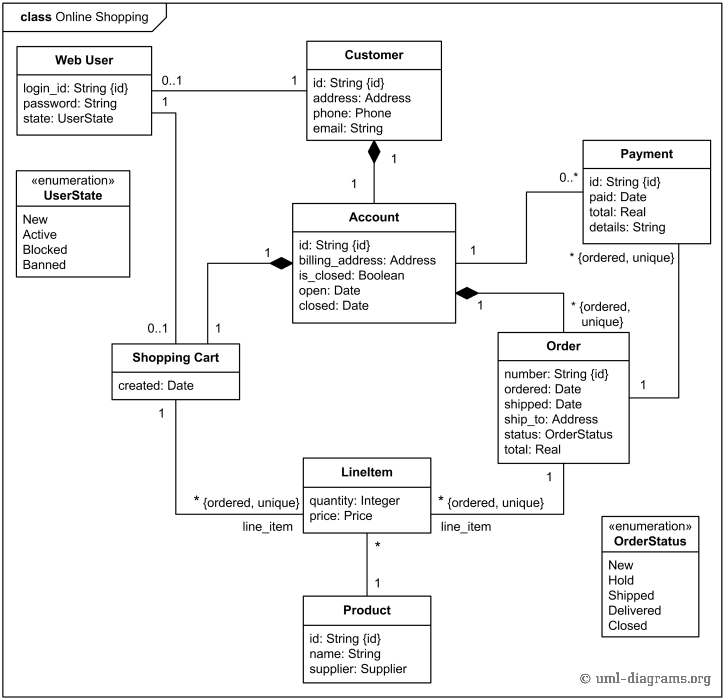
\includegraphics[width=12cm]{images/diagrams/domain-model-uml-ecommerce.png}
  \caption{Example of a Domain Model Class Diagram for an eCommerce website}
  \label{fig:domain-model-uml-ecommerce}
\end{figure}
\vspace{0.5cm}

Although some partial \textit{IFMLModel} representations for the Madison Island eCommerce platform have already been introduced in \ref{navigational-modeling-for-the-web}, in this subsection we explore the most important ones in more detail and with a broader approach that is not strictly related to the navigational modeling. Our final goal is to build an \textit{IFMLModel} which would represent the main pages and website interactions, taking advantage of the IFML metamodel described just above.

\subsubsection{Global overview}

The Madison Island Interaction Model is formed by a different combination of \textit{IFMLWindow} elements connected through \textit{IFMLAction}s reacting to distinct \textit{Events} with different \textit{ParameterBindings}. The detail of the modeling is contextual to the purpose of this work. Consequently, we have limited the inclusion of the possible interactions and elements presented on the website to the \textit{IFMLModel}. In so doing, we keep the model design lightweight and reduce its complexity. Overall, the main \textit{IFMLWindow} standalone nodes have been described with more detail when compared to other shared \textit{ViewContainer} elements, such as the Header and the Footer. In Figure \ref{fig:ifml-before-global}, a visual representation of the IFMLDiagram corresponding to the main \textit{IFMLModel} for the Madison Island eCommerce platform is presented.

\vspace{0.5cm}
\begin{figure}[H]
  \centering
    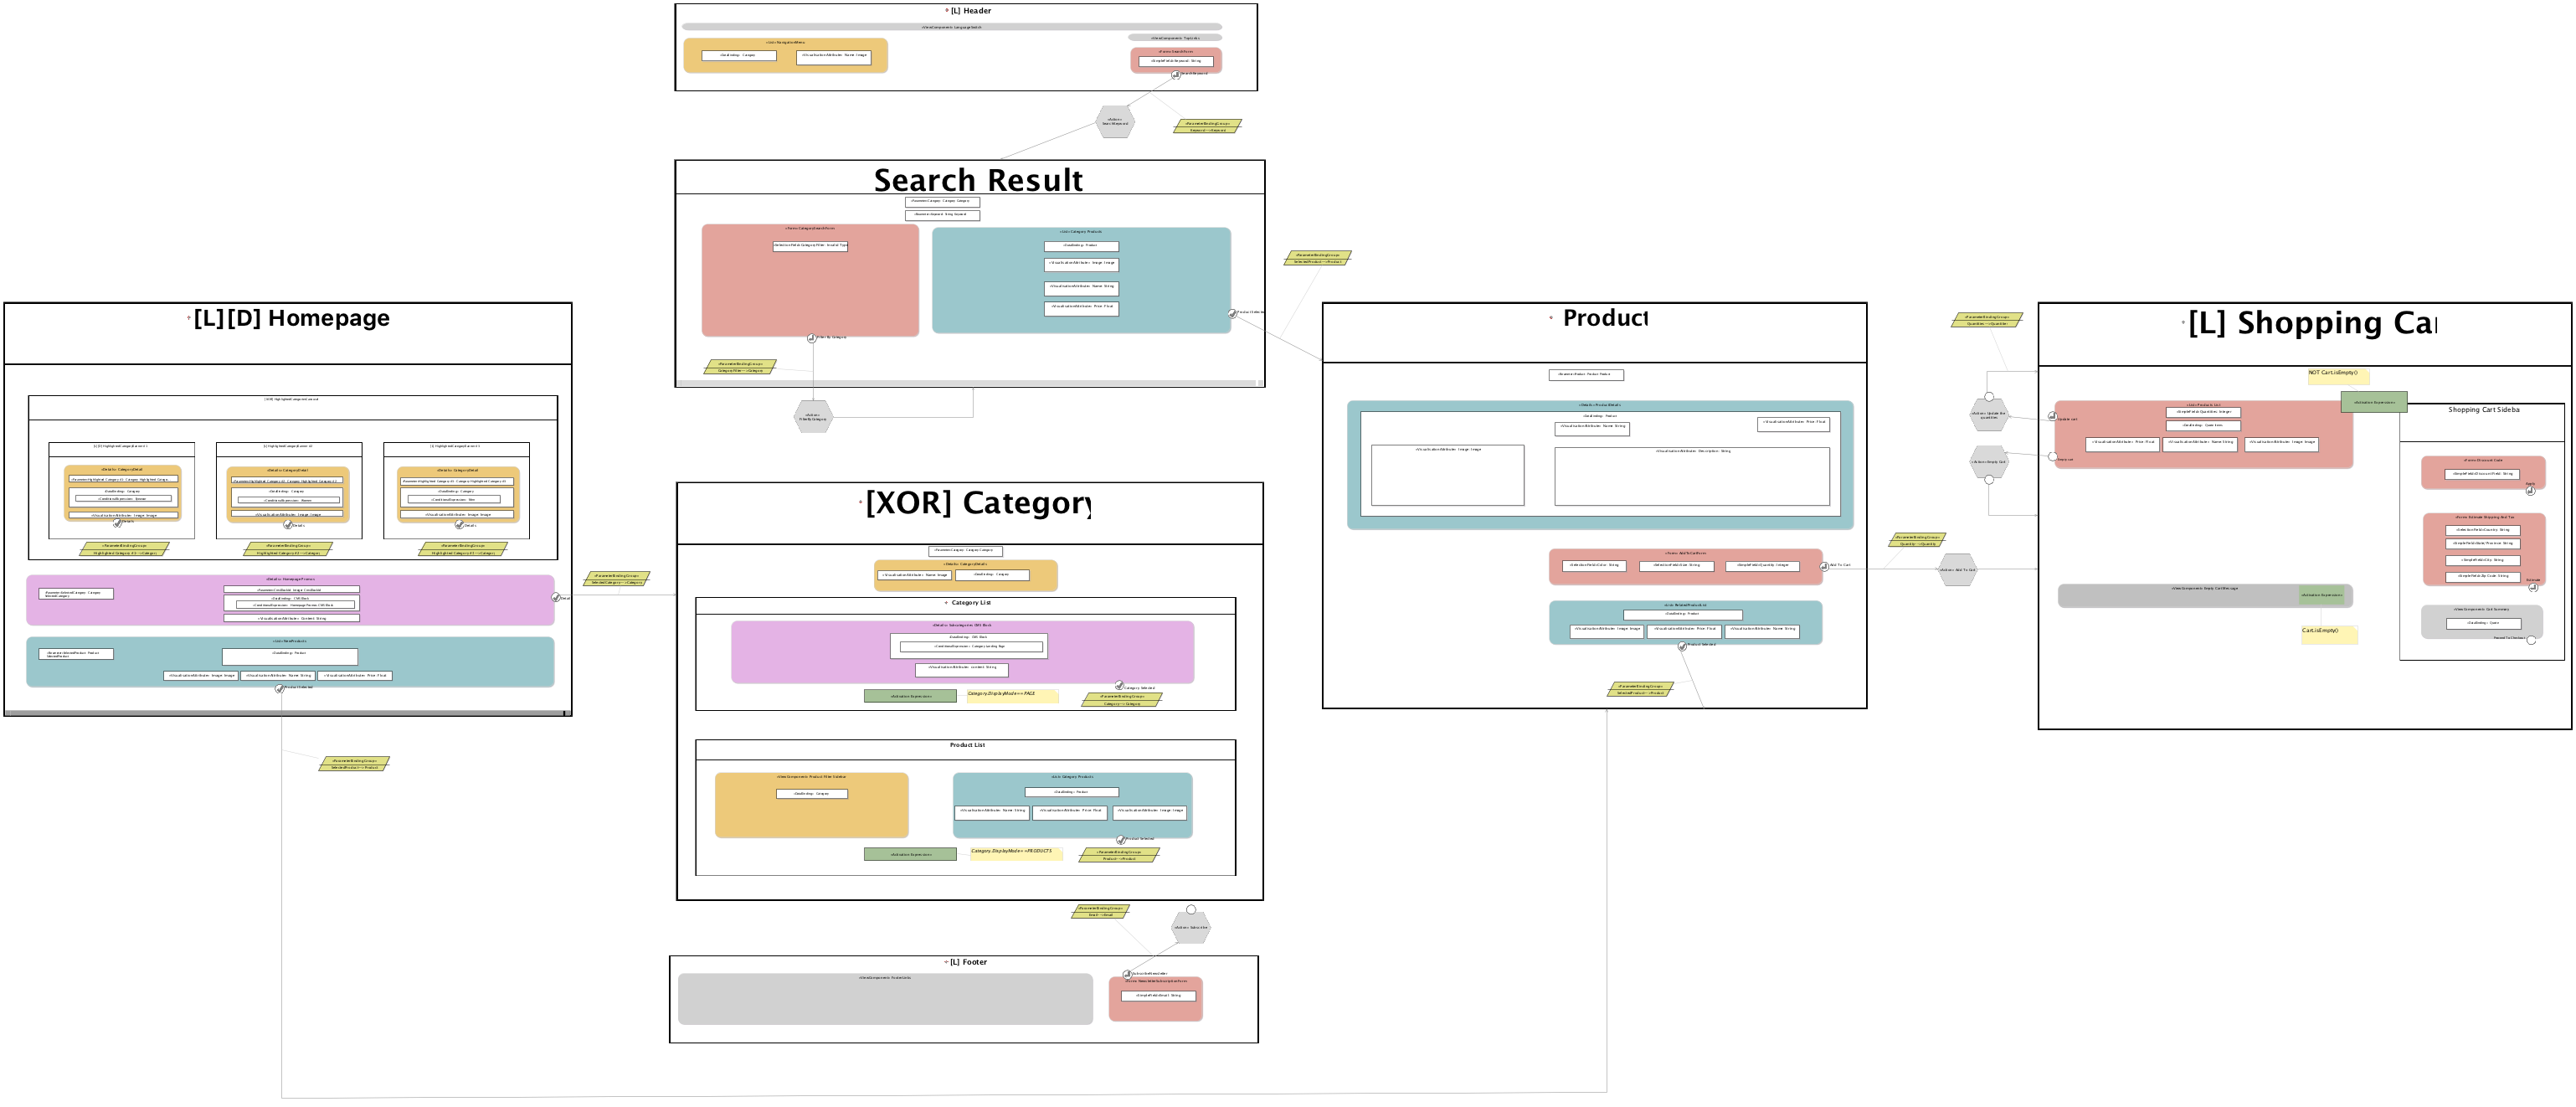
\includegraphics[height=6.5cm] {images/diagrams/before/ifml-global.png}
  \caption{Main Madison Island IFML Diagram overview}
  \label{fig:ifml-before-global}
\end{figure}
\vspace{0.5cm}
\newpage
\subsubsection{Homepage}

The Madison Island Interaction Model for the Homepage (Figure \ref{fig:desktop-before-homepage} and \ref{fig:ifml-before-homepage}) is composed by a parent \textit{IFMLWindow} element, which contains three children elements: another \textit{IFMLWindow} for the Highlighted Categories Carousel, a \textit{Detail View Component} for the Homepage promos CMS Block, and a \textit{List View Component} for the New Products sections that is bound to the Product Entity of the \textit{Domain Model} . The parent HighlightedCategoriesCarousel \textit{IFMLWindow} has the \textit{isXOR} property set to true, representing three exclusive main configurations for the initial screen within the carousel mechanism. Each \textit{Data Binding} within all these banner components is limited by a \textit{Conditional Expressions} defining the instance of the content to show.

\vspace{0.5cm}
\begin{figure}[H]
  \centering
    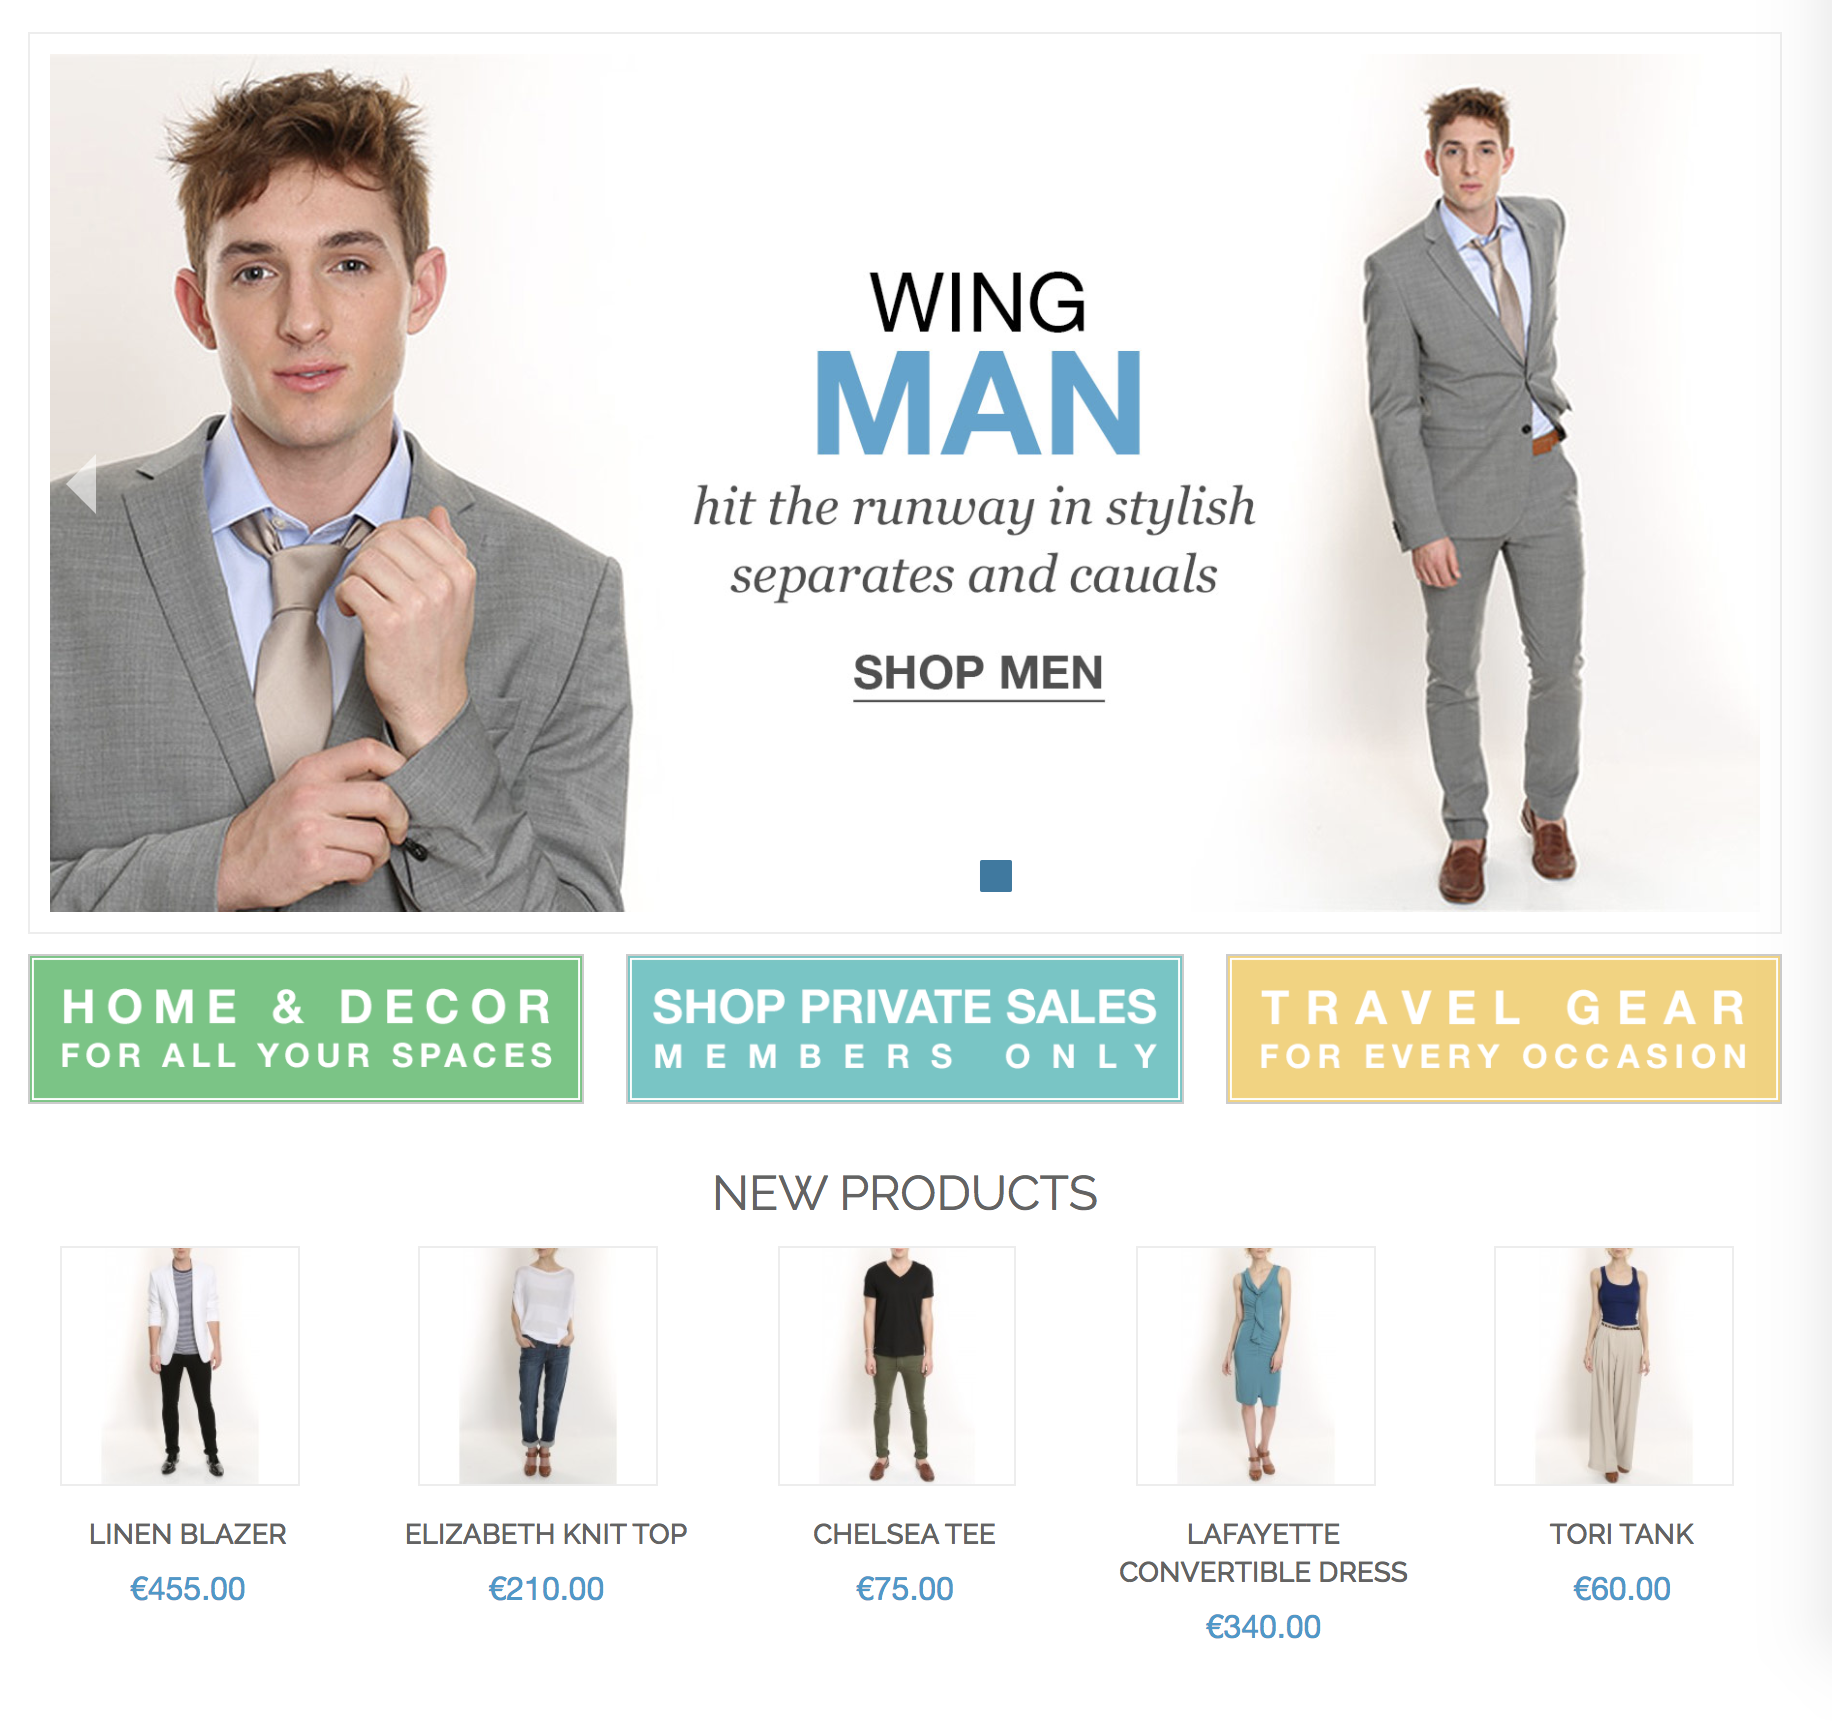
\includegraphics[width=14cm]{images/diagrams/before/desktop-homepage.png}
  \caption{Homepage Desktop Version}
  \label{fig:desktop-before-homepage}
\end{figure}
\vspace{0.5cm}

\begin{figure}[H]
  \centering
    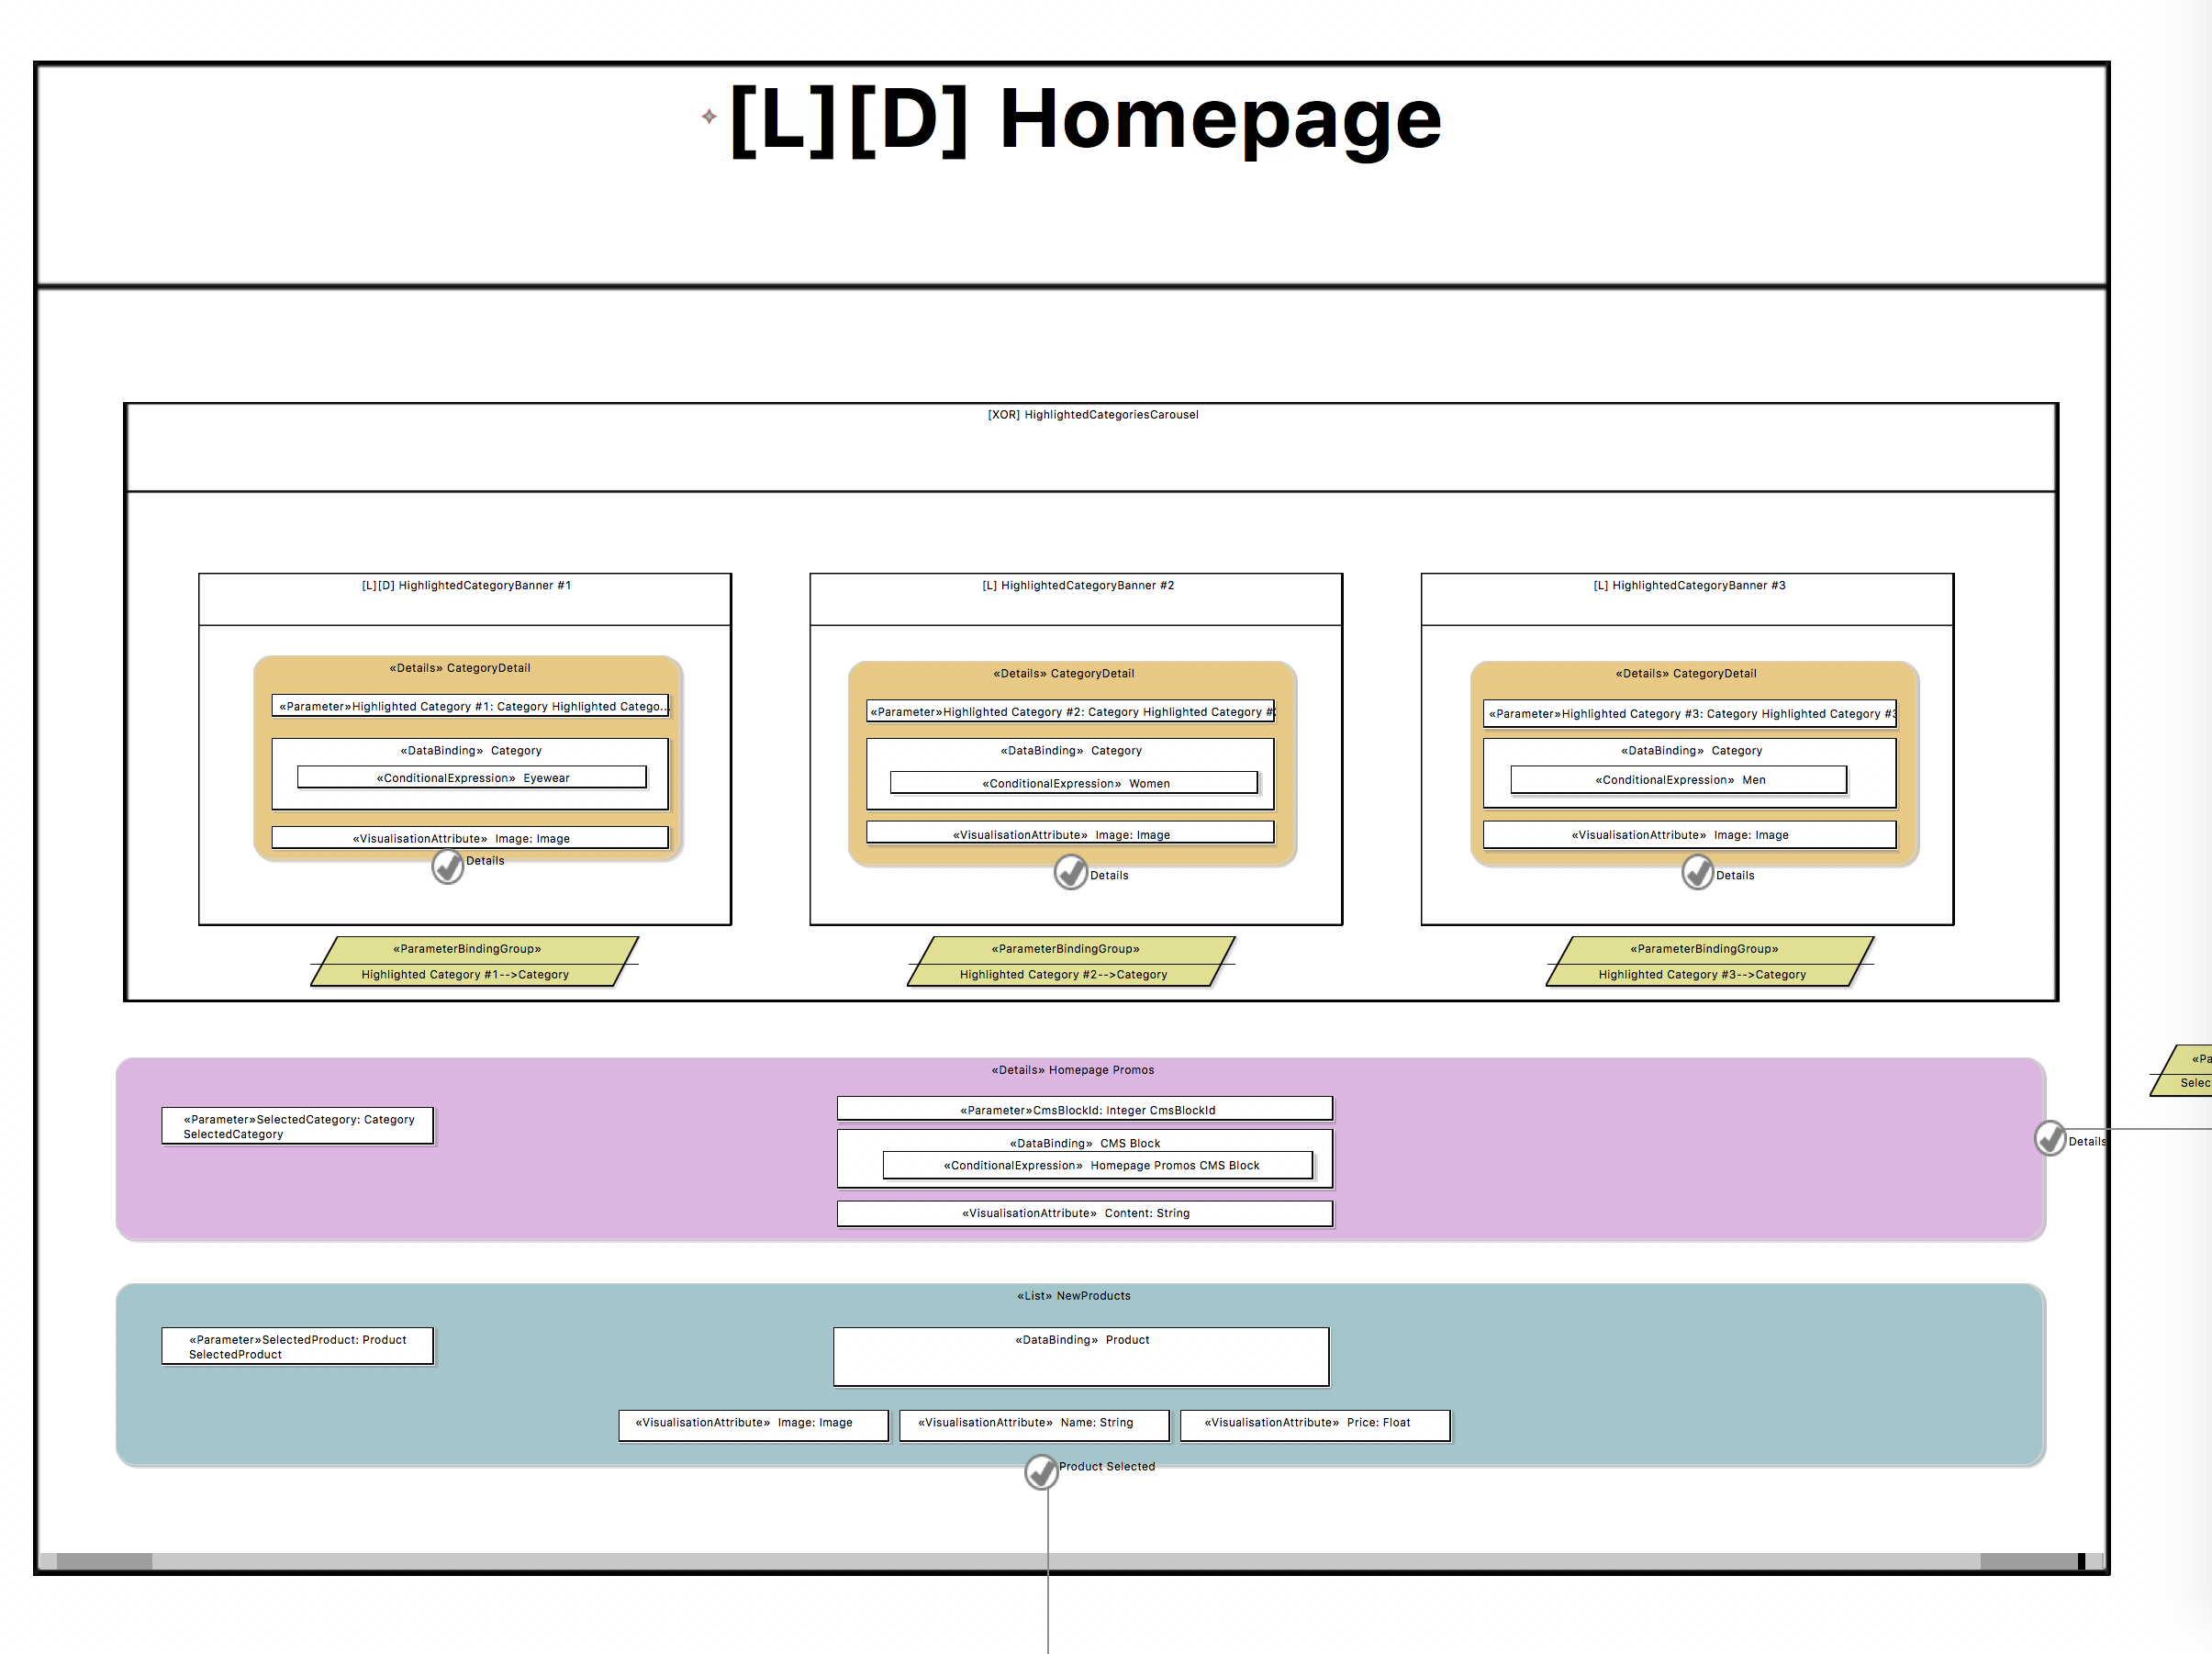
\includegraphics[width=14cm]{images/diagrams/before/ifml-homepage.png}
  \caption{Homepage IFML Diagram}
  \label{fig:ifml-before-homepage}
\end{figure}
\vspace{0.5cm}

The following snippet of code is an extract from the \textit{IFMLModel} for the first HighlighedCategoryBanner \textit{View Container} element: 
\vspace{0.5cm}
\lstset{language=XML}
\begin{lstlisting} 
      <viewElements xsi:type="ext:Details"  name="CategoryDetail">
        <parameters  name="Highlighted Category #1" direction="inout">
          <constraints  language="SQL" body="Category.ID=18"/>
        </parameters>
        <viewElementEvents xsi:type="ext:OnSelectEvent"  name="Details" viewElement="//@interactionFlowModel/@interactionFlowModelElements.0/@viewElements.0/@viewElements.0">
          <outInteractionFlows xsi:type="core:NavigationFlow"  targetInteractionFlowElement="//@interactionFlowModel/@interactionFlowModelElements.6">
            <parameterBindingGroup >
              <parameterBindings  sourceParameter="//@interactionFlowModel/@interactionFlowModelElements.0/@viewElements.0/@viewElements.0/@viewElements.0/@parameters.0" targetParameter="//@interactionFlowModel/@interactionFlowModelElements.6/@parameters.0"/>
            </parameterBindingGroup>
          </outInteractionFlows>
        </viewElementEvents>
        <viewComponentParts xsi:type="core:DataBinding"  name="Category" uniformResourceIdentifier="">
          <subViewComponentParts xsi:type="core:ConditionalExpression"  language="SQL" body="Category.ID=18" name="Eyewear"/>
        </viewComponentParts>
        <viewComponentParts xsi:type="core:VisualizationAttribute"  name="Image" featureConcept="//@domainModel/@domainElements.4"/>
      </viewElements>
    </viewElements>
\end{lstlisting}

The above snippet belongs to a more complex \textit{IFMLModel} hierarchy, as shown in \ref{fig:ifml-before-hierarchy-homepage}.

\vspace{0.5cm}
\begin{figure}[H]
  \centering
    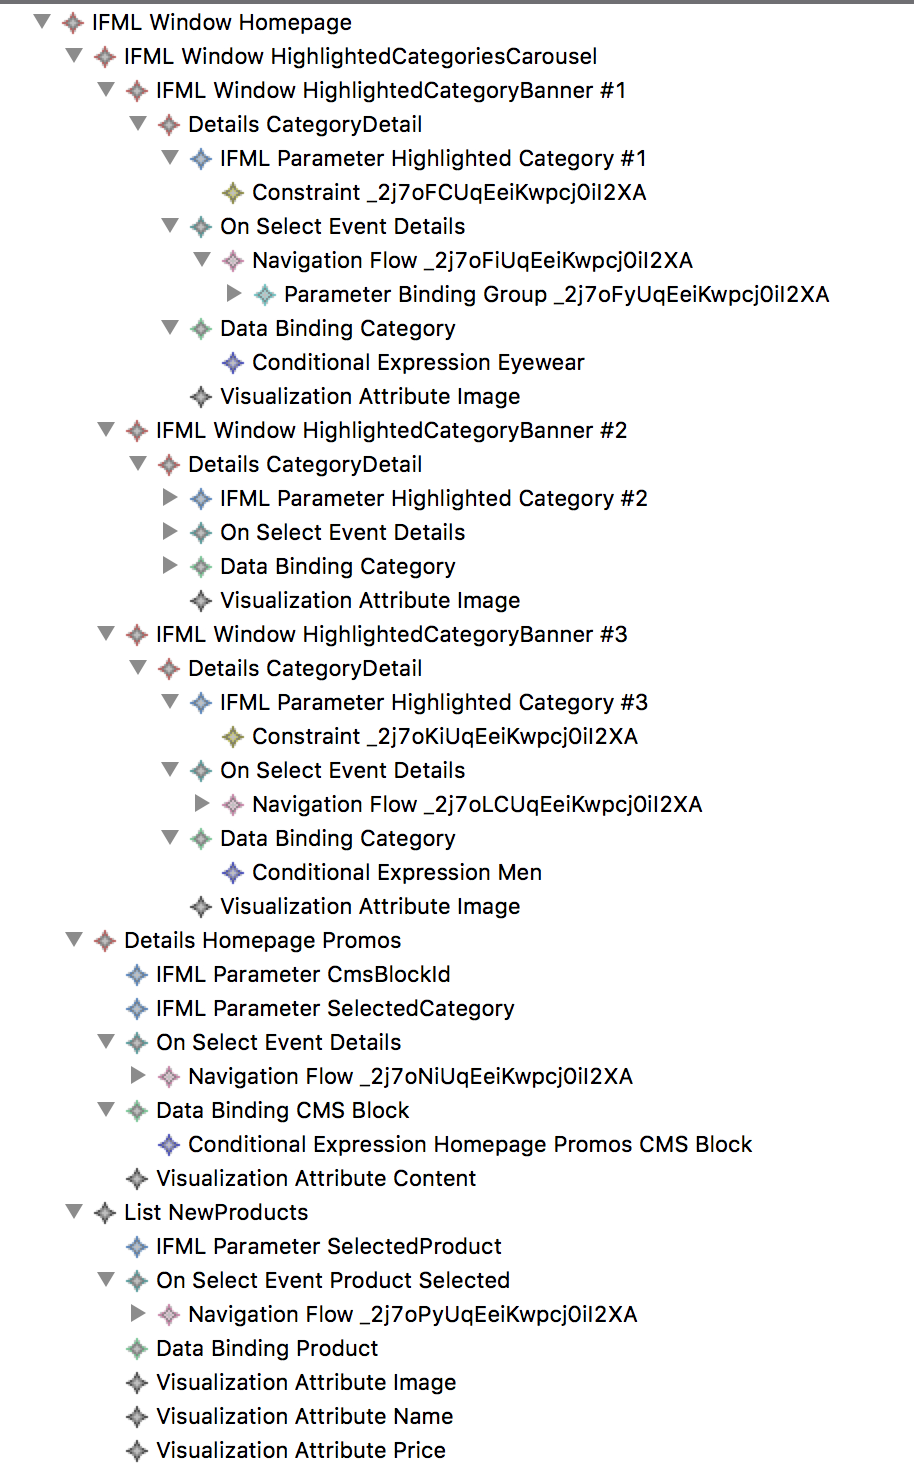
\includegraphics[width=10cm]{images/diagrams/before/ifml-hierarchy-homepage.png}
  \caption{Interaction Flow Homepage Model in EMF}
  \label{fig:ifml-before-hierarchy-homepage}
\end{figure}
\vspace{0.5cm}

\newpage
\subsubsection{Category Page}

The Madison Island Interaction Model for the Category Page (Figure \ref{fig:desktop-before-category} and \ref{fig:ifml-before-category}) is composed by a parent \textit{IFMLWindow} element with a true-ish \textit{isXOR} property, which presents information about the current category on the top of the page. Depending on the display mode property for the Category Entity, the user can be presented with two different \textit{View Containers} that are respectively activated using different \textit{Activation Expressions} based on the value of the property itself. Whilst the first scenario presents a \textit{Detail View Component} attached to a linked CMS Block, the second option shows two children view components representing both the filter sidebar and the products listing section with this last one having multiple \textit{Visualization Attribute} children nodes. These nodes indicate that the user is presented with an image used as thumbnail, a name and a price for each product belonging to the category shown.

\vspace{0.5cm}
\begin{figure}[H]
  \centering
  \subfloat[Category Page with Display Mode PAGE]{{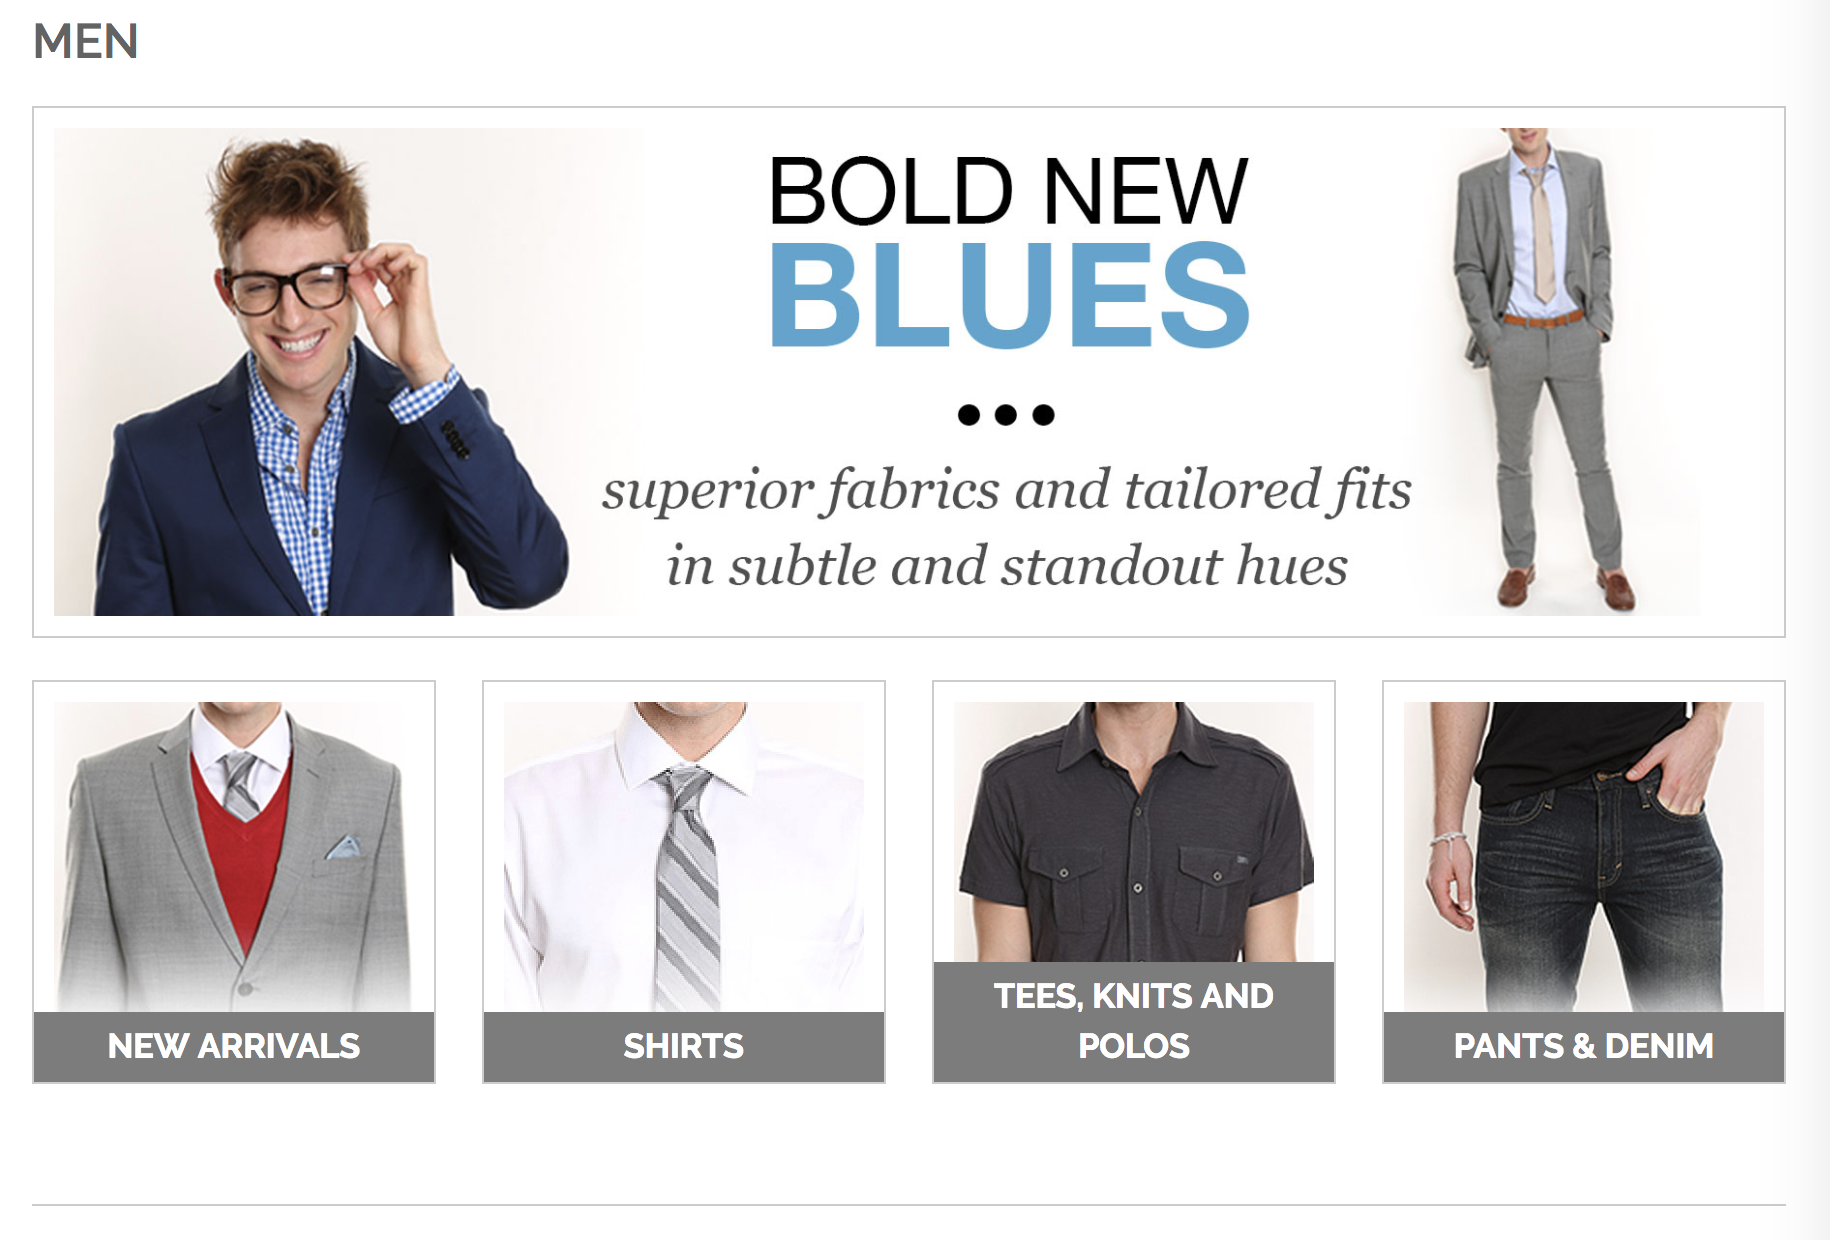
\includegraphics[width=8cm]{images/diagrams/before/desktop-category1.png} }}%
  \qquad
  \subfloat[Category Page with Display Mode PRODUCTS]{{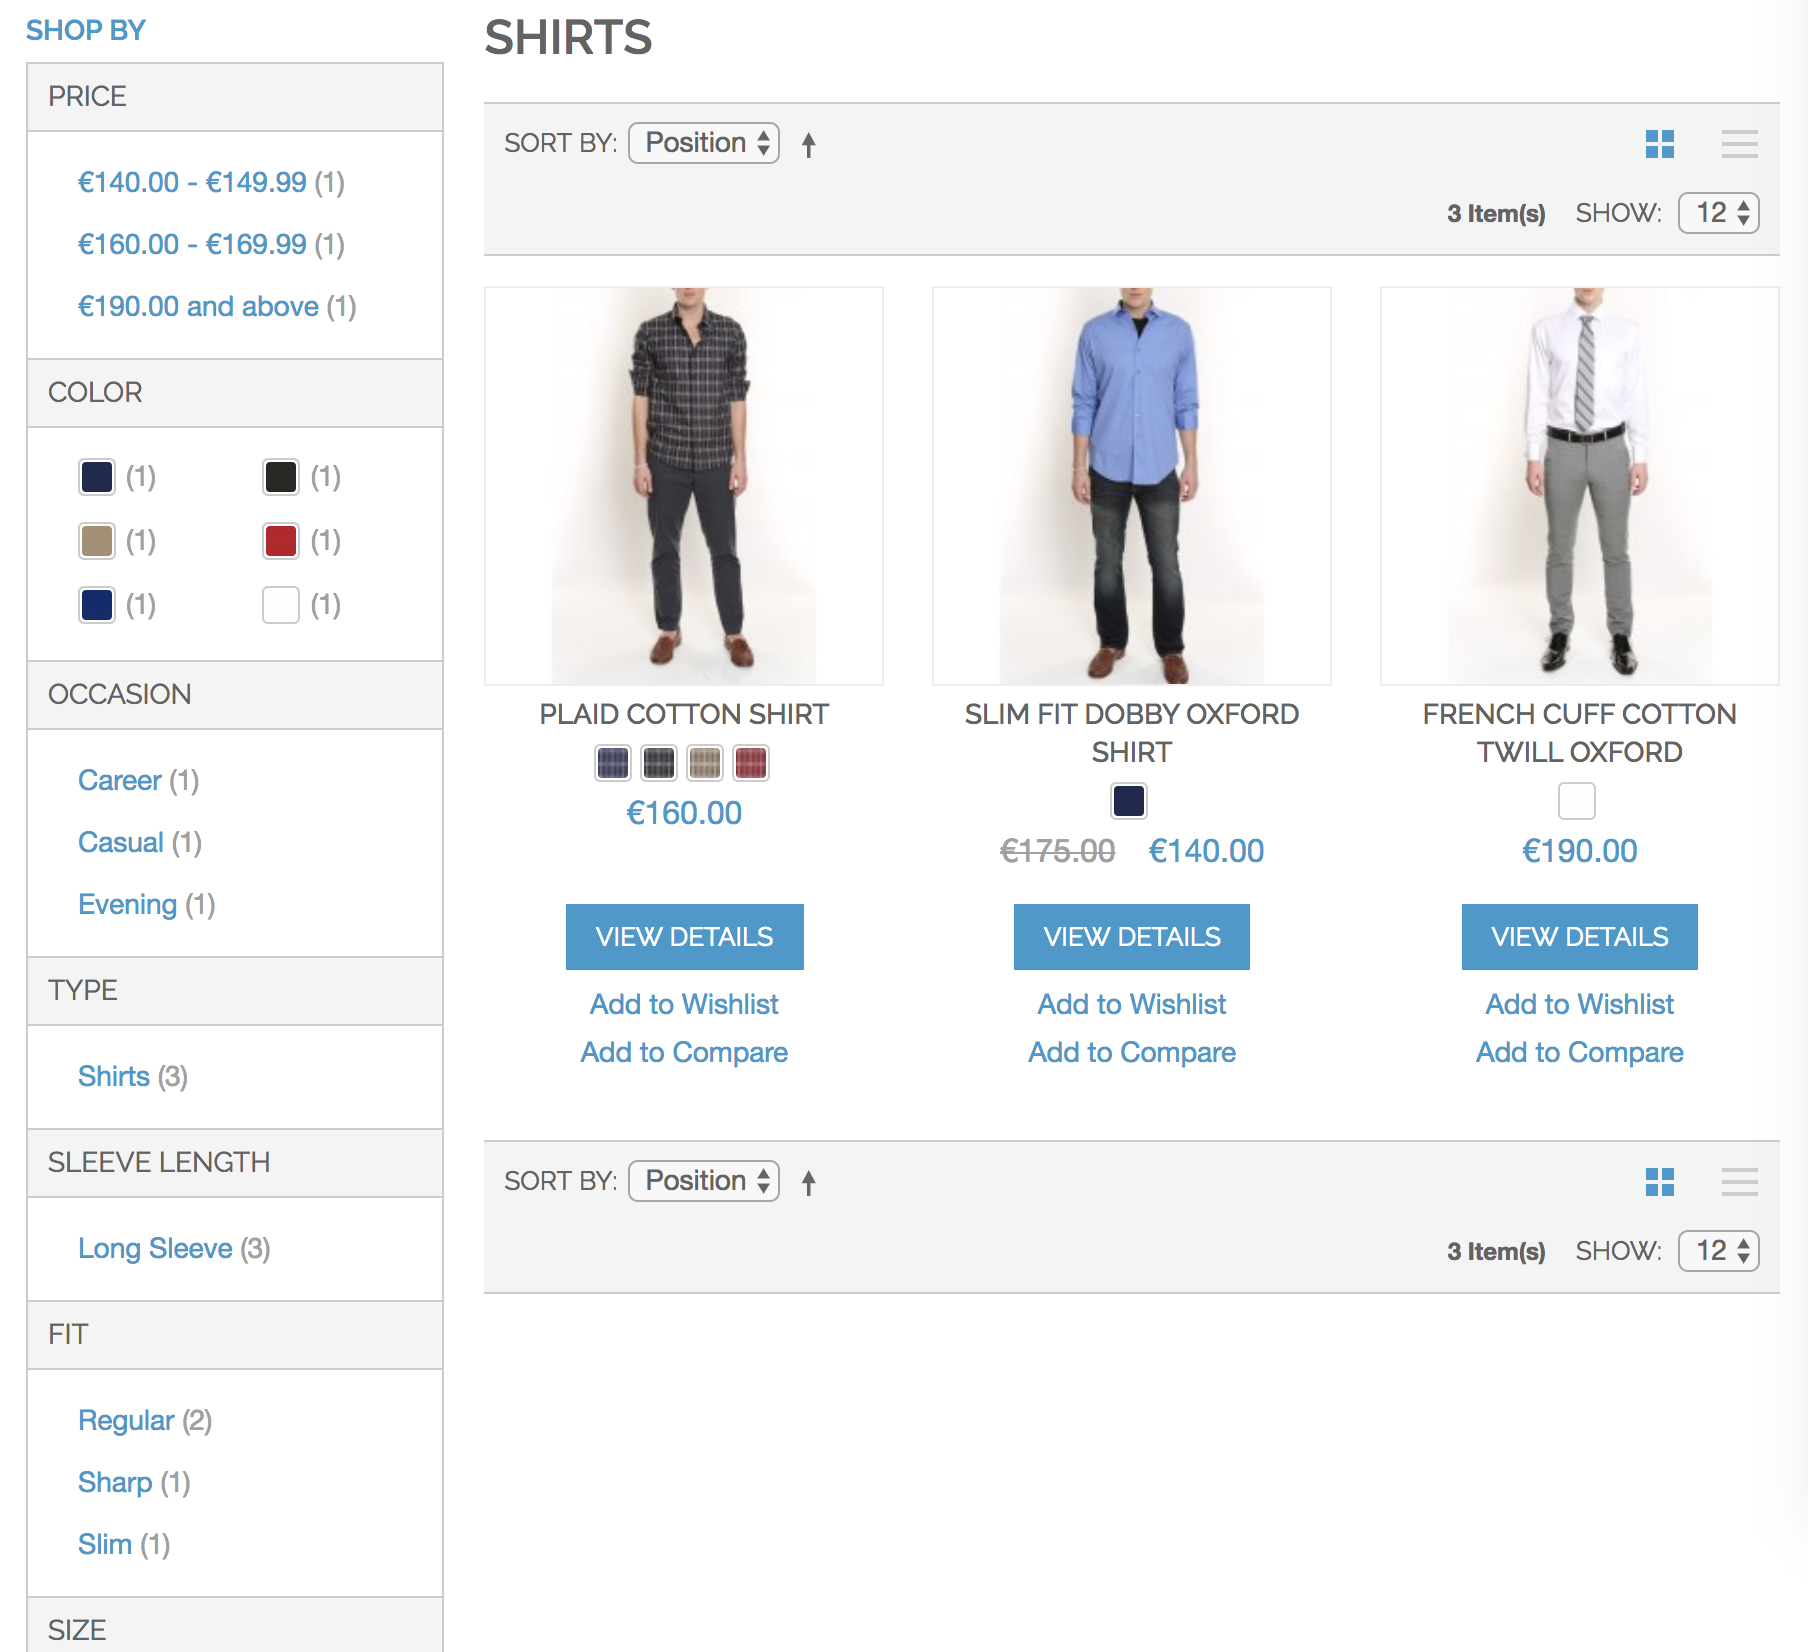
\includegraphics[width=8cm]{images/diagrams/before/desktop-category2.png} }}%
  \caption{Category Desktop Versions}%
  \label{fig:desktop-before-category}%
\end{figure}

\begin{figure}[H]
  \centering
    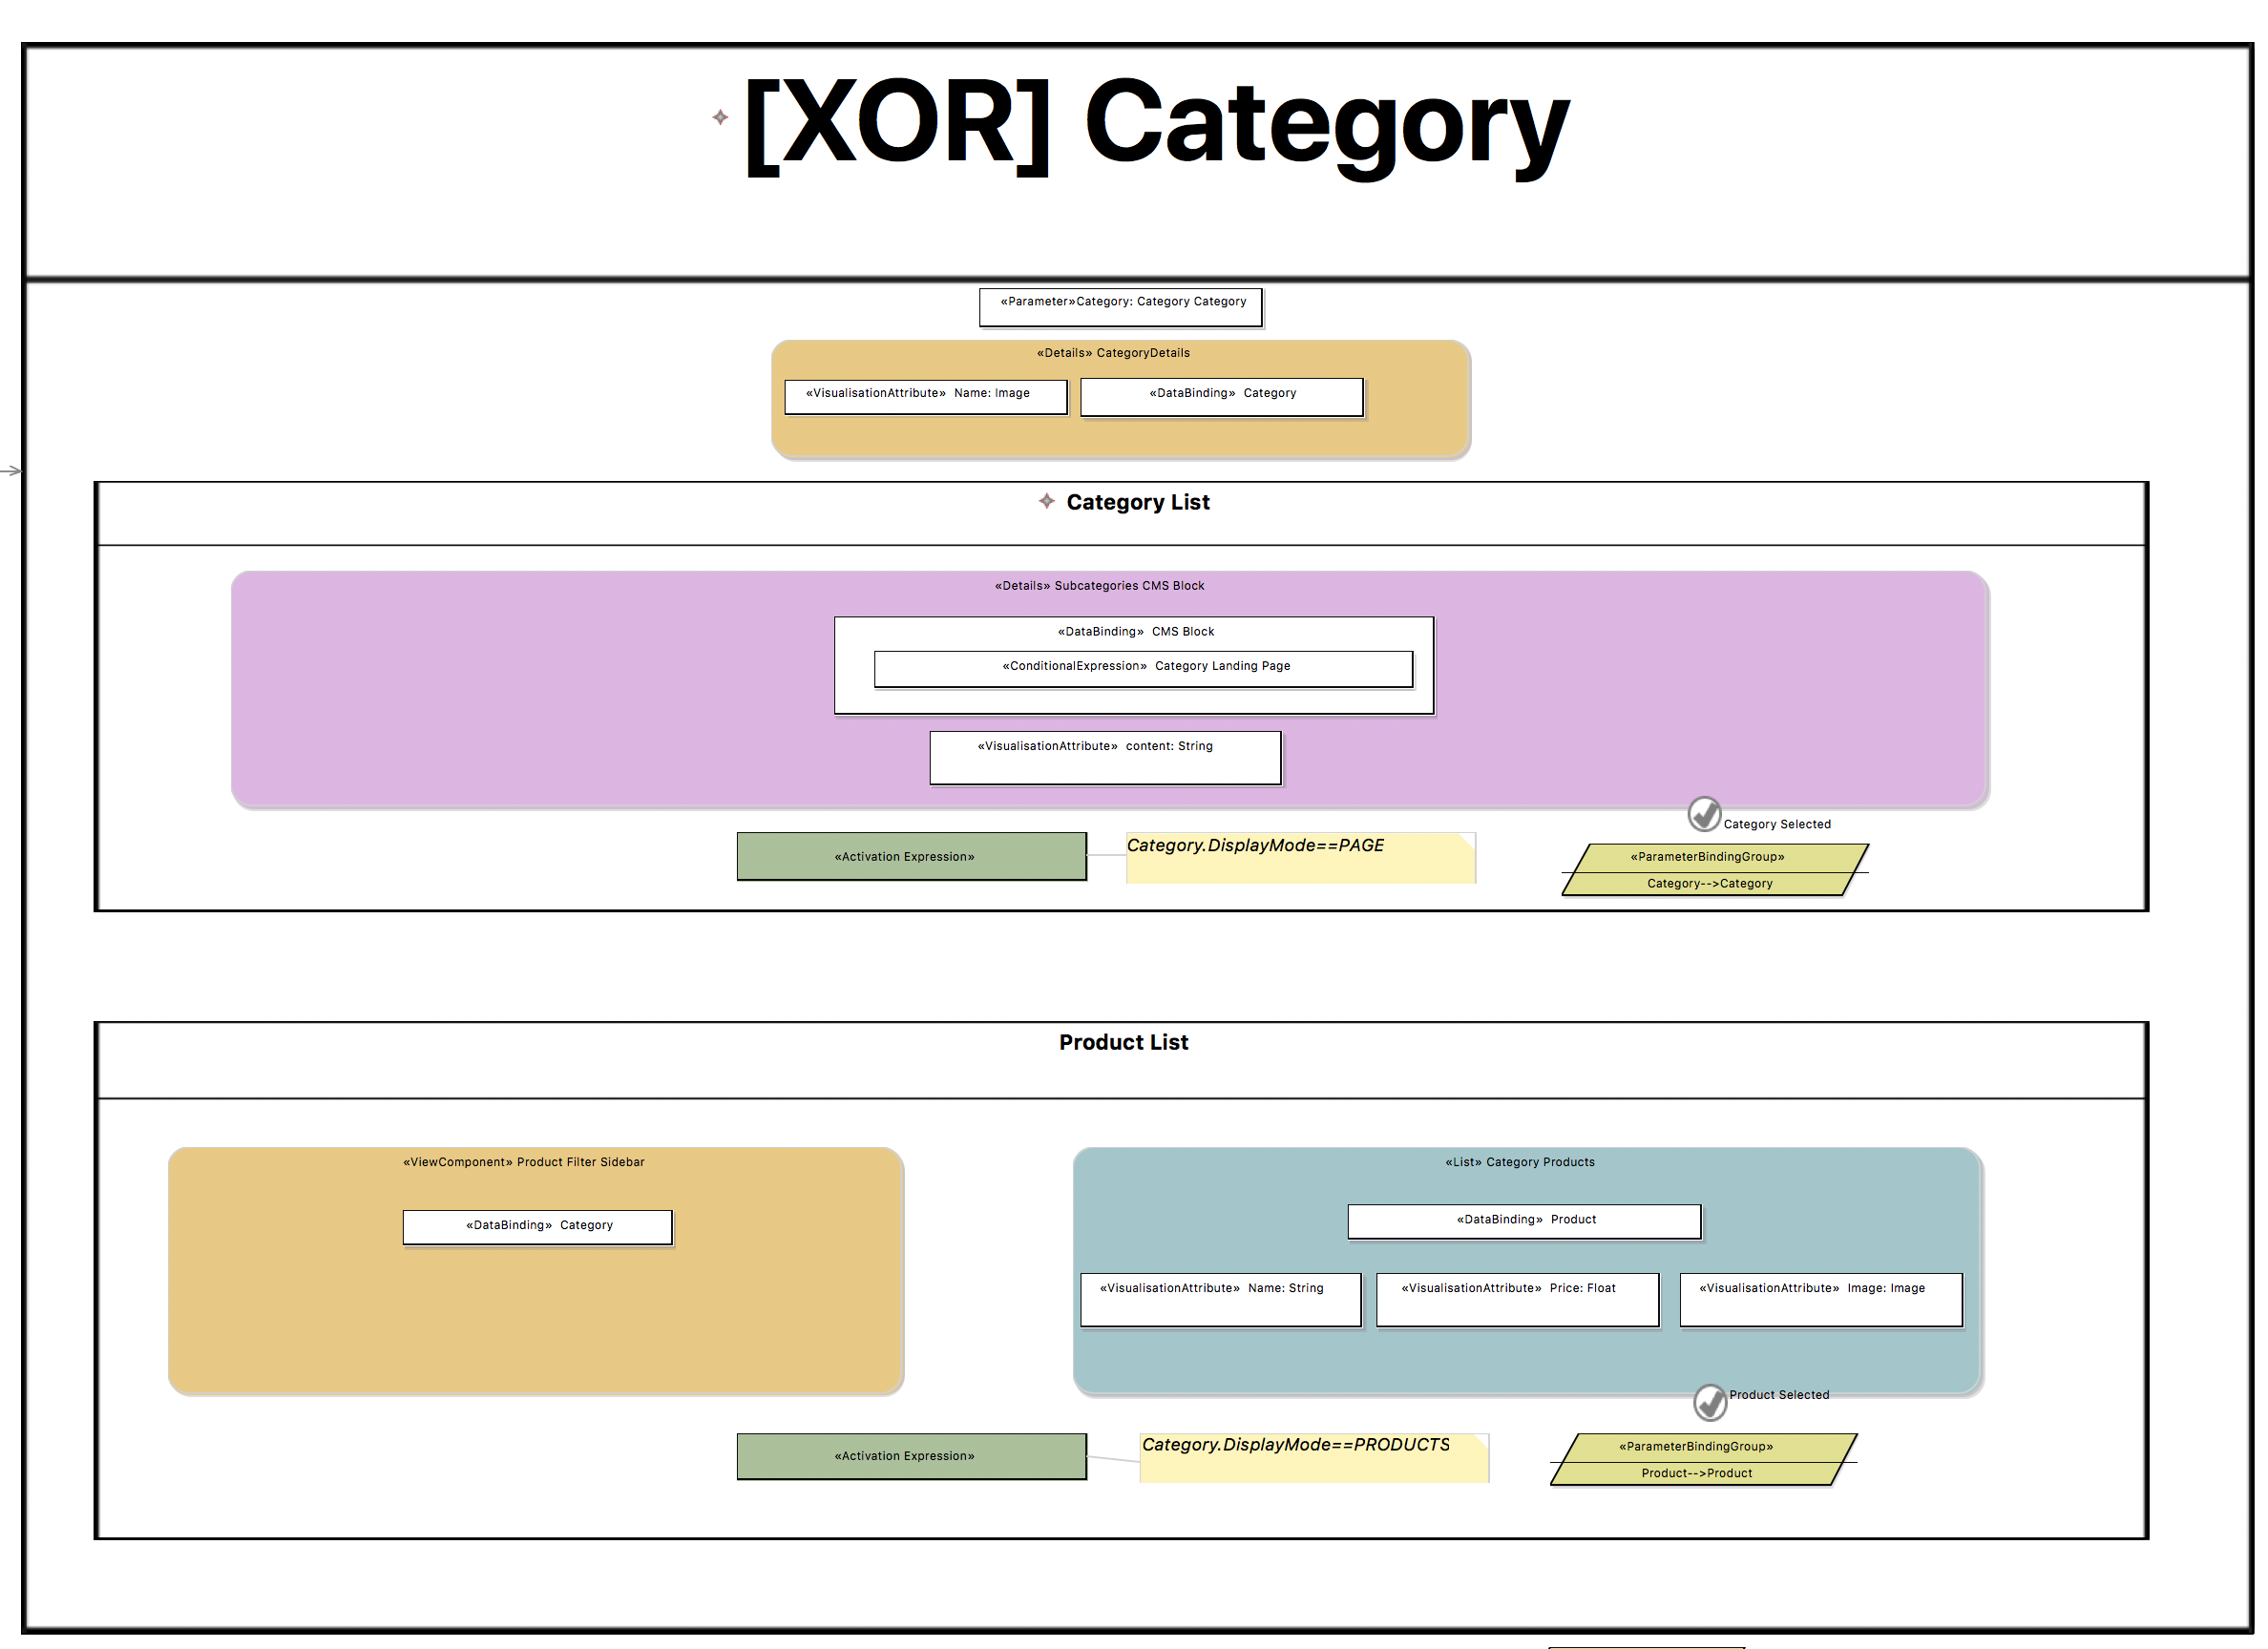
\includegraphics[width=14cm]{images/diagrams/before/ifml-category.png}
  \caption{Category IFML Diagram}
  \label{fig:ifml-before-category}
\end{figure}
\vspace{0.5cm}

The \textit{IFMLModel} code for the first Category Products List element we have just described takes this form: 
\vspace{0.5cm}
\lstset{language=XML}
\begin{lstlisting} 
    <viewElements xsi:type="ext:List"  name="Category Products">
    <viewElementEvents xsi:type="ext:OnSelectEvent"  name="Product Selected" viewElement="//@interactionFlowModel/@interactionFlowModelElements.6/@viewElements.1/@viewElements.0">
      <outInteractionFlows xsi:type="core:NavigationFlow"  targetInteractionFlowElement="//@interactionFlowModel/@interactionFlowModelElements.1">
        <parameterBindingGroup >
          <parameterBindings  sourceParameter="//@interactionFlowModel/@interactionFlowModelElements.1/@parameters.0" targetParameter="//@interactionFlowModel/@interactionFlowModelElements.1/@parameters.0"/>
        </parameterBindingGroup>
      </outInteractionFlows>
    </viewElementEvents>
    <viewComponentParts xsi:type="core:DataBinding"  name="Product" domainConcept="//@domainModel/@domainElements.3">
      <conditionalExpression  language="SQL" body="Category IN Product.Categories" name="Category Products"/>
    </viewComponentParts>
    <viewComponentParts xsi:type="core:VisualizationAttribute"  name="Image" featureConcept="//@domainModel/@domainElements.7"/>
    <viewComponentParts xsi:type="core:VisualizationAttribute"  name="Name" featureConcept="//@domainModel/@domainElements.8"/>
    <viewComponentParts xsi:type="core:VisualizationAttribute"  name="Price" featureConcept="//@domainModel/@domainElements.9"/>
  </viewElements>
  <viewElements xsi:type="core:ViewComponent"  name="Product Filter Sidebar">
    <viewComponentParts xsi:type="core:DataBinding"  name="Category"/>
  </viewElements>
</viewElements>
\end{lstlisting}

The full expanded model hierarchy for the \textit{IFMLWindow} Category element is shown in Figure~\ref{fig:ifml-before-hierarchy-category}.

\vspace{0.5cm}
\begin{figure}[H]
  \centering
    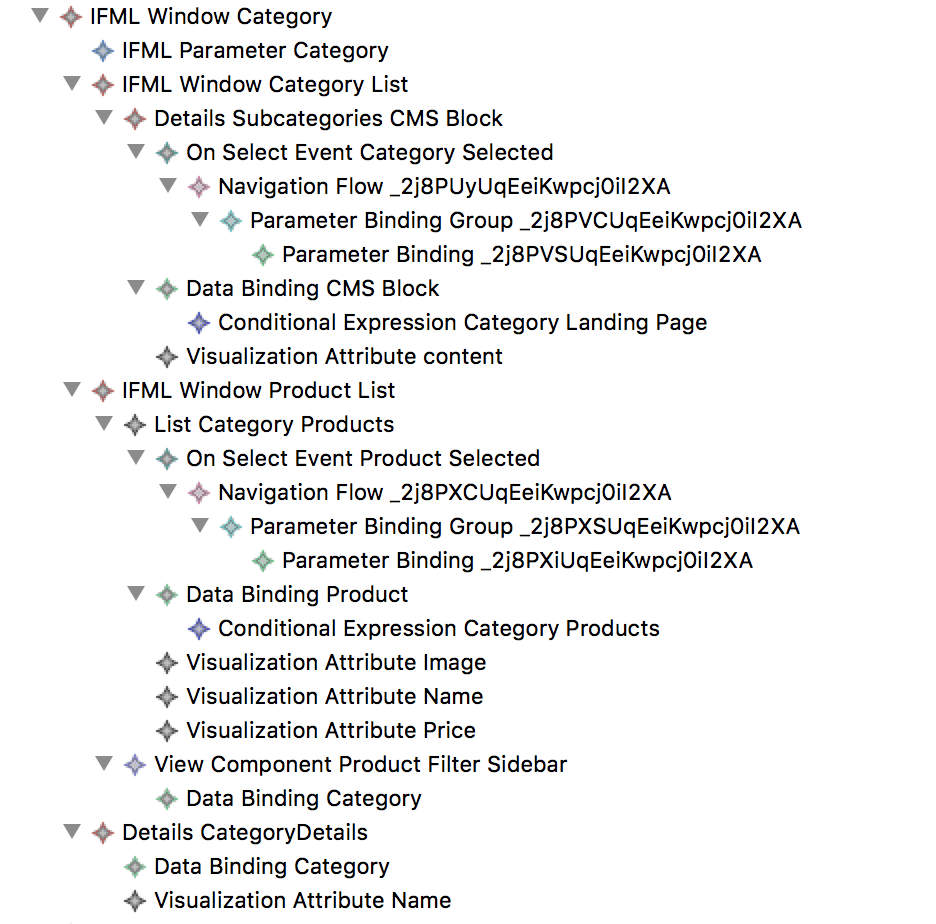
\includegraphics[width=13cm]{images/diagrams/before/ifml-hierarchy-category.png}
  \caption{Interaction Flow Category Model in EMF}
  \label{fig:ifml-before-hierarchy-category}
\end{figure}
\vspace{0.5cm}

\newpage
\subsubsection{Product Page}

The Madison Island Interaction Model for the Product page (Figure \ref{fig:desktop-before-product} and \ref{fig:ifml-before-product}) is mainly built with a single \textit{IFMLWindow} element that contains different types of \textit{View Component} nodes, the main one being a \textit{Detail View Component} instance bound to the current product data entity. The other two elements are the single \textit{Form View Component} describing the Add to Cart section and its possible interactions, and the \textit{List View Component} holding the information for the Related Product widget.

\vspace{0.5cm}
\begin{figure}[H]
  \centering
    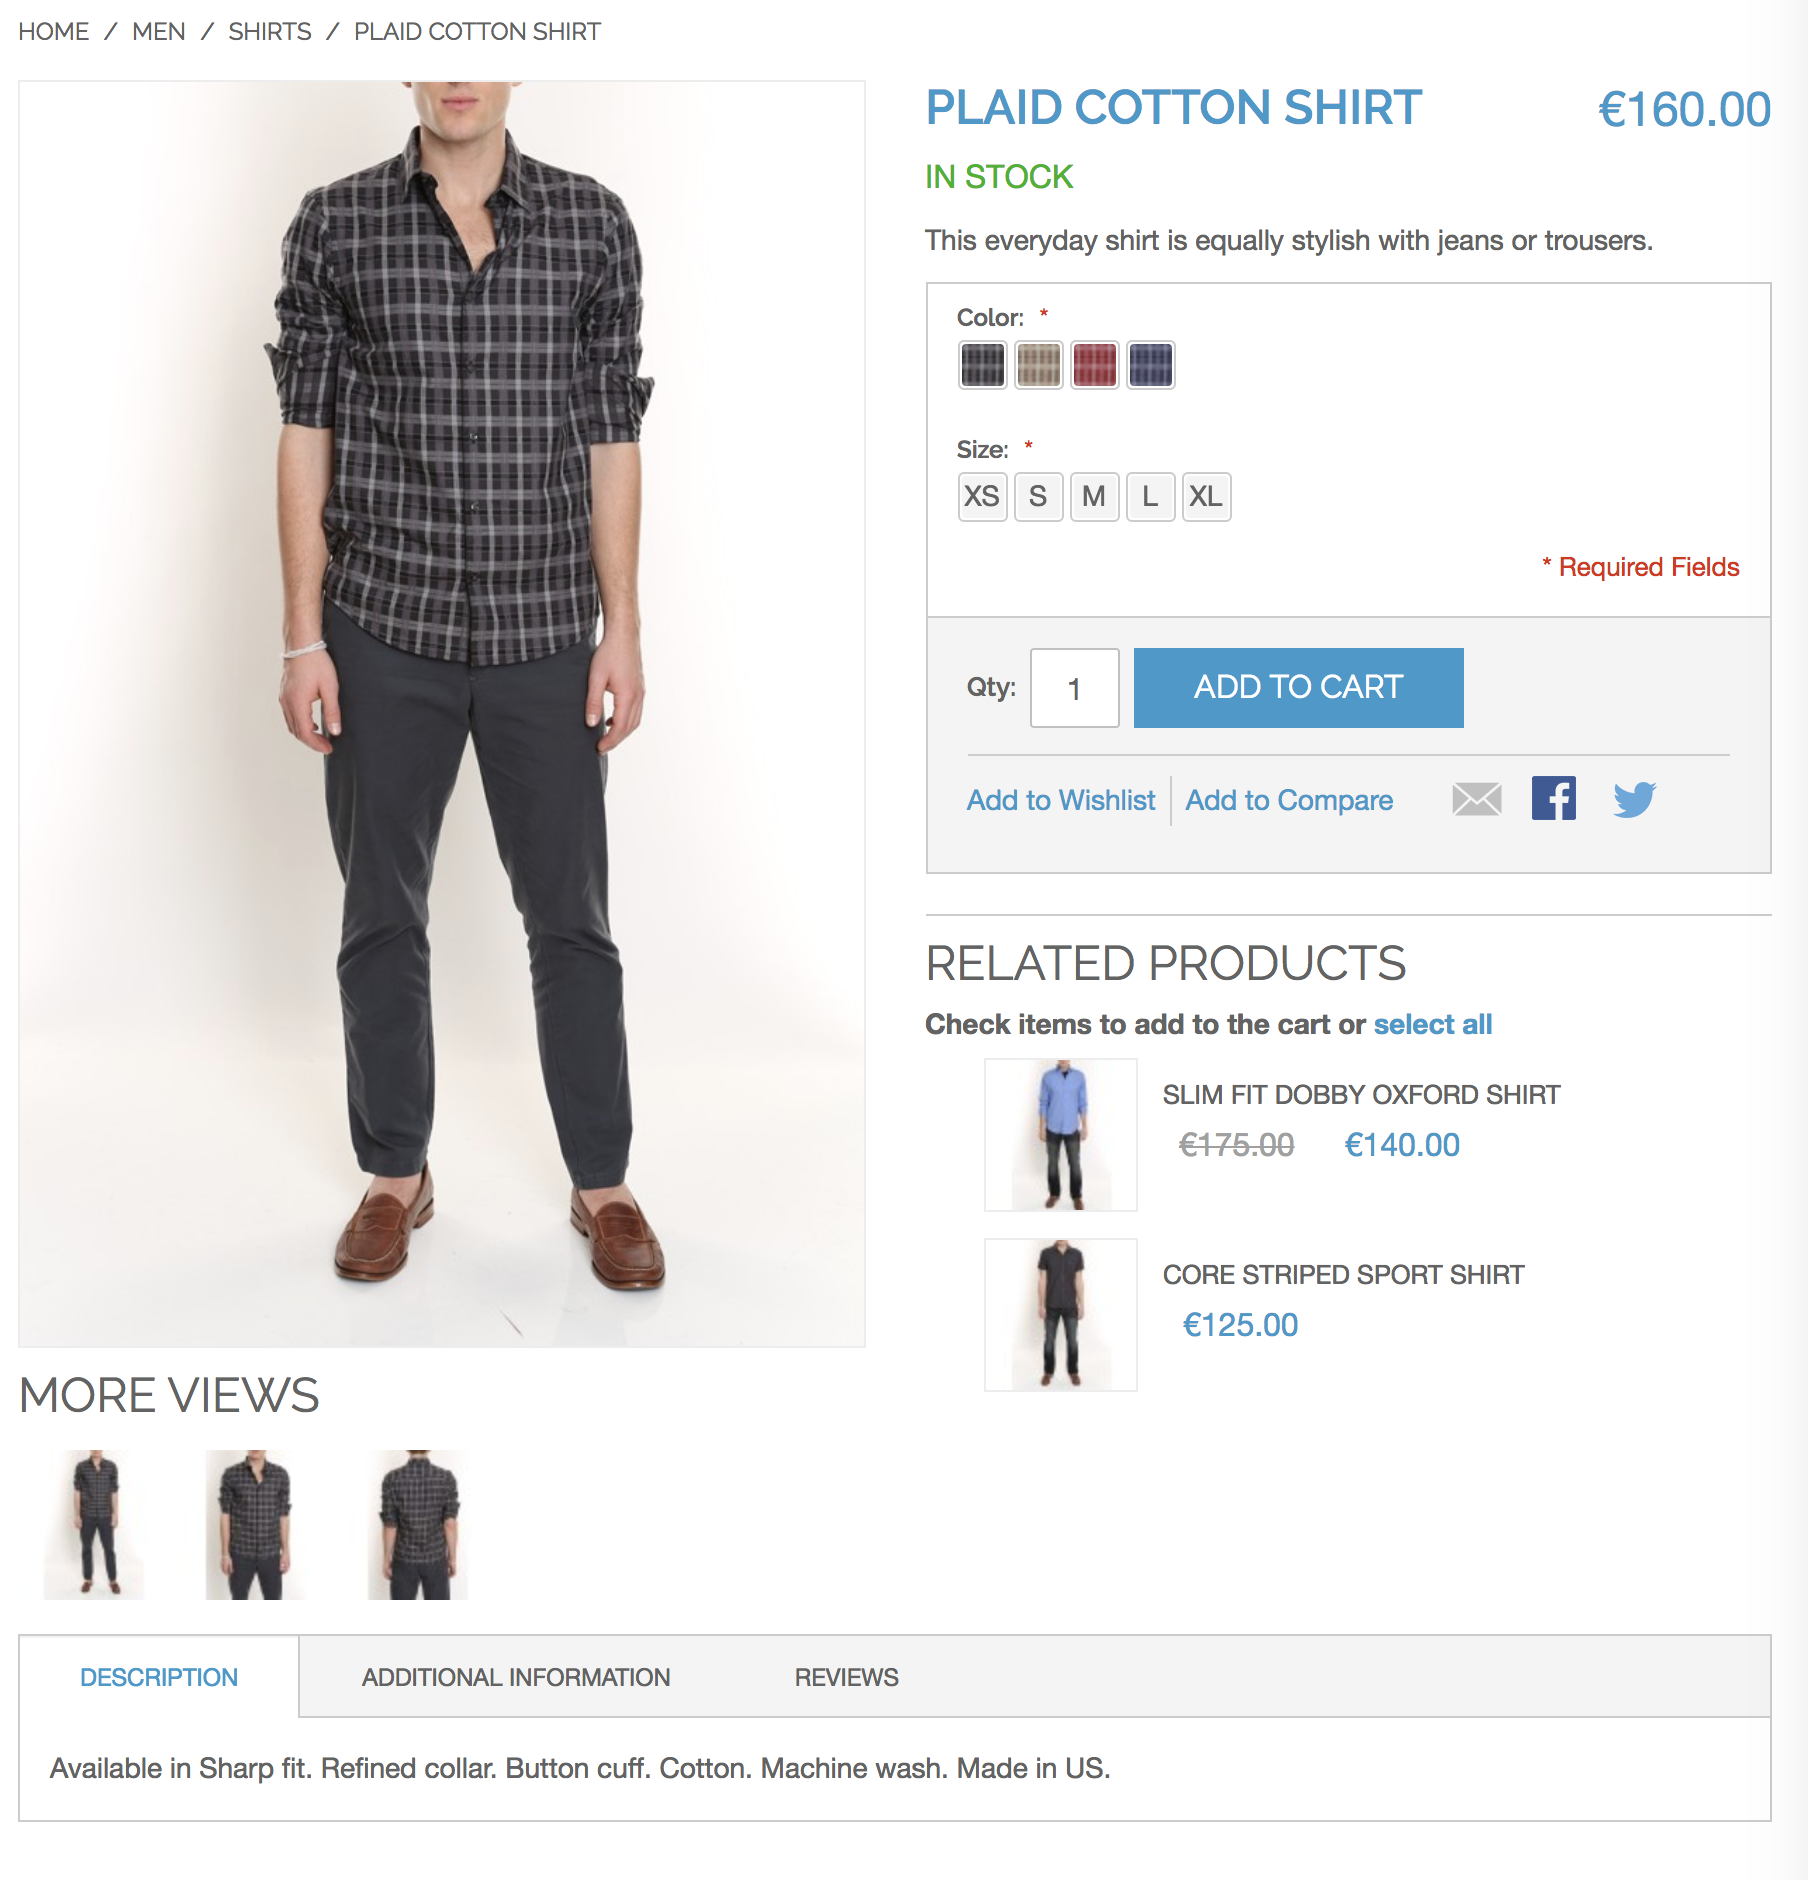
\includegraphics[width=14cm]{images/diagrams/before/desktop-product.png}
  \caption{Product Page Desktop Version}
  \label{fig:desktop-before-product}
\end{figure}

\vspace{0.5cm}
\begin{figure}[H]
  \centering
    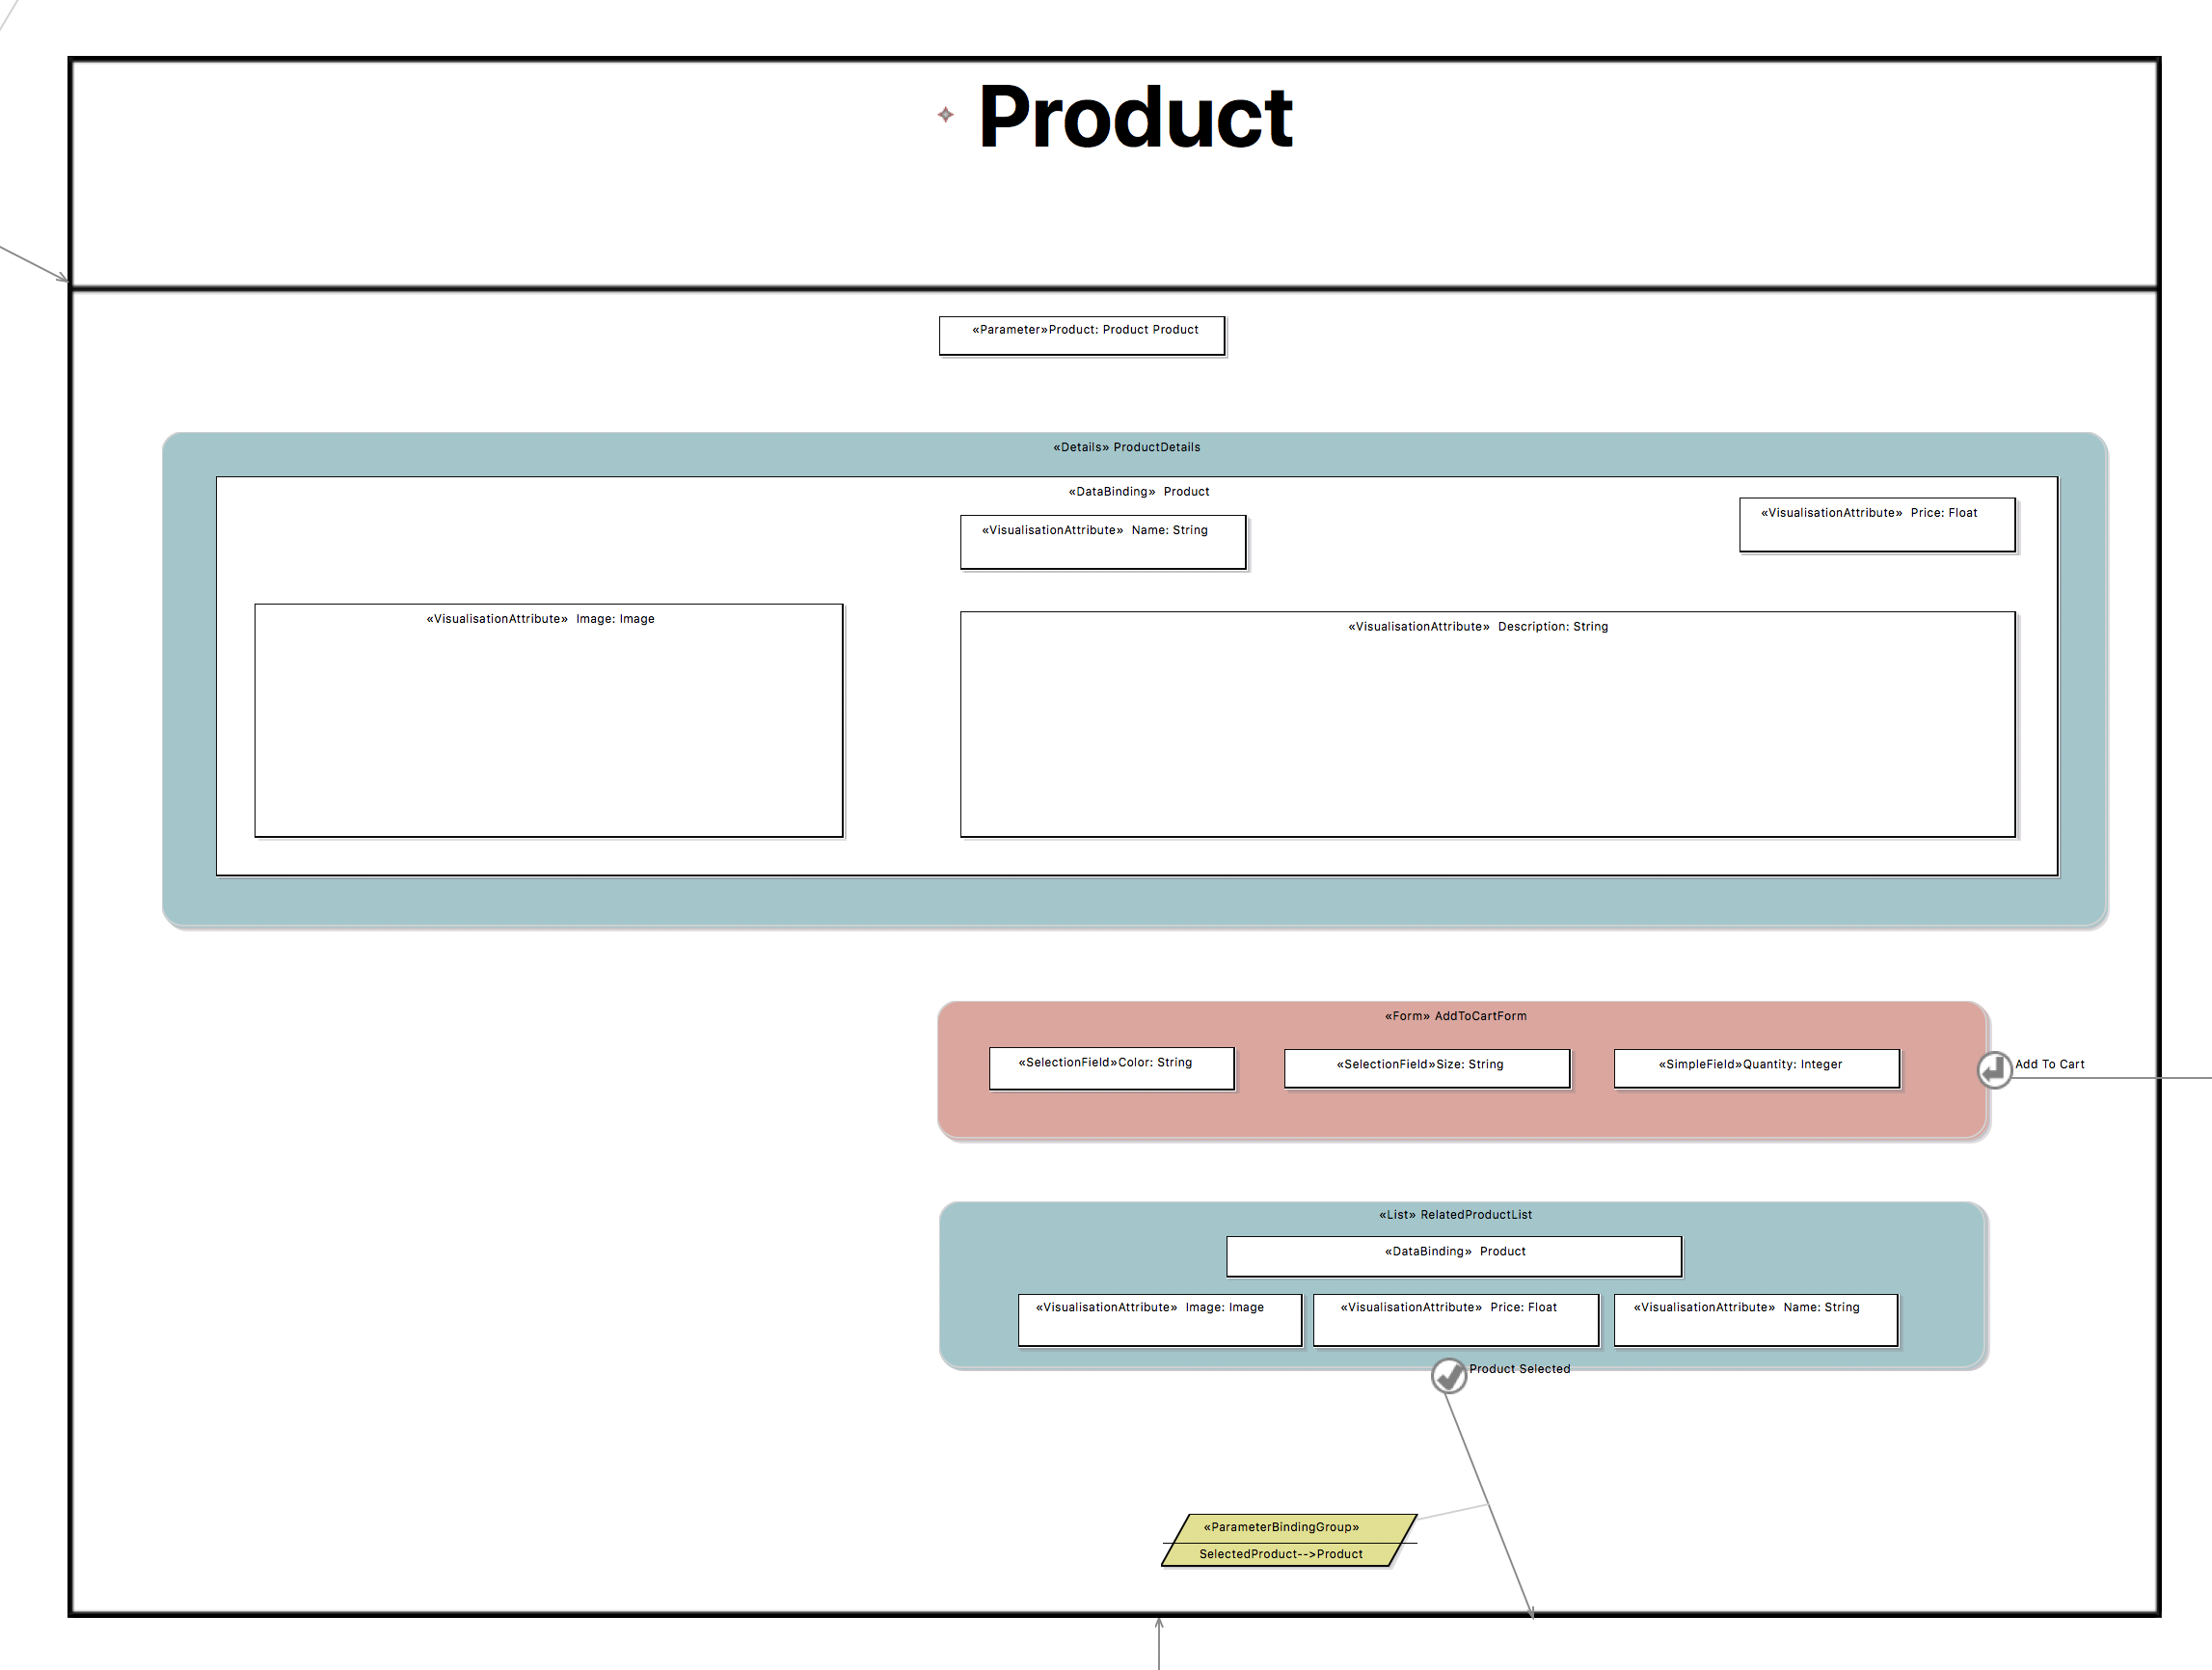
\includegraphics[width=14cm]{images/diagrams/before/ifml-product.png}
  \caption{Product Page IFML Diagram}
  \label{fig:ifml-before-product}
\end{figure}
\vspace{0.5cm}

The structure of the model just outlined produces the following \textit{IFMLModel} code:
\vspace{0.5cm}
\lstset{language=XML}
\begin{lstlisting} 
    <interactionFlowModelElements xsi:type="ext:IFMLWindow"  name="Product" inInteractionFlows="//@interactionFlowModel/@interactionFlowModelElements.1/@viewElements.2/@viewElementEvents.0/@outInteractionFlows.0 //@interactionFlowModel/@interactionFlowModelElements.0/@viewElements.2/@viewElementEvents.0/@outInteractionFlows.0 //@interactionFlowModel/@interactionFlowModelElements.10/@viewElements.0/@viewElementEvents.0/@outInteractionFlows.0 //@interactionFlowModel/@interactionFlowModelElements.6/@viewElements.1/@viewElements.0/@viewElementEvents.0/@outInteractionFlows.0">
      <parameters  name="Product" />
      <viewElements xsi:type="ext:Details"  name="ProductDetails">
        <viewComponentParts xsi:type="core:DataBinding"  name="Product" uniformResourceIdentifier="">
          <subViewComponentParts xsi:type="core:VisualizationAttribute"  name="Price" featureConcept="//@domainModel/@domainElements.9"/>
          <subViewComponentParts xsi:type="core:VisualizationAttribute"  name="Image" featureConcept="//@domainModel/@domainElements.7"/>
          <subViewComponentParts xsi:type="core:VisualizationAttribute"  name="Name" featureConcept="//@domainModel/@domainElements.8"/>
          <subViewComponentParts xsi:type="core:VisualizationAttribute"  name="Description" featureConcept="//@domainModel/@domainElements.10"/>
        </viewComponentParts>
      </viewElements>
      <viewElements xsi:type="ext:Form"  name="AddToCartForm">
        <viewElementEvents xsi:type="ext:OnSubmitEvent"  name="Add To Cart" viewElement="//@interactionFlowModel/@interactionFlowModelElements.1/@viewElements.1">
          <outInteractionFlows xsi:type="core:NavigationFlow"  targetInteractionFlowElement="//@interactionFlowModel/@interactionFlowModelElements.9">
            <parameterBindingGroup >
              <parameterBindings  sourceParameter="//@interactionFlowModel/@interactionFlowModelElements.1/@viewElements.1/@viewComponentParts.2" targetParameter="//@interactionFlowModel/@interactionFlowModelElements.1/@viewElements.1/@viewComponentParts.2"/>
            </parameterBindingGroup>
          </outInteractionFlows>
        </viewElementEvents>
        <viewComponentParts xsi:type="ext:SelectionField"  name="Color" />
        <viewComponentParts xsi:type="ext:SelectionField"  name="Size" />
        <viewComponentParts xsi:type="ext:SimpleField"  name="Quantity" />
      </viewElements>
      <viewElements xsi:type="ext:List"  name="RelatedProductList">
        <viewElementEvents xsi:type="ext:OnSelectEvent"  name="Product Selected" viewElement="//@interactionFlowModel/@interactionFlowModelElements.1/@viewElements.2">
          <outInteractionFlows xsi:type="core:NavigationFlow"  targetInteractionFlowElement="//@interactionFlowModel/@interactionFlowModelElements.1">
            <parameterBindingGroup >
              <parameterBindings  sourceParameter="//@interactionFlowModel/@interactionFlowModelElements.0/@viewElements.2/@parameters.0" targetParameter="//@interactionFlowModel/@interactionFlowModelElements.1/@parameters.0"/>
            </parameterBindingGroup>
          </outInteractionFlows>
        </viewElementEvents>
        <viewComponentParts xsi:type="core:DataBinding"  name="Product"/>
        <viewComponentParts xsi:type="core:VisualizationAttribute"  name="Image" featureConcept="//@domainModel/@domainElements.7"/>
        <viewComponentParts xsi:type="core:VisualizationAttribute"  name="Name" featureConcept="//@domainModel/@domainElements.8"/>
        <viewComponentParts xsi:type="core:VisualizationAttribute"  name="Price" featureConcept="//@domainModel/@domainElements.9"/>
      </viewElements>
    </interactionFlowModelElements>
\end{lstlisting}


The model representation of this product page structure is shown in Figure \ref{fig:ifml-before-hierarchy-product}

\vspace{0.5cm}
\begin{figure}[H]
  \centering
    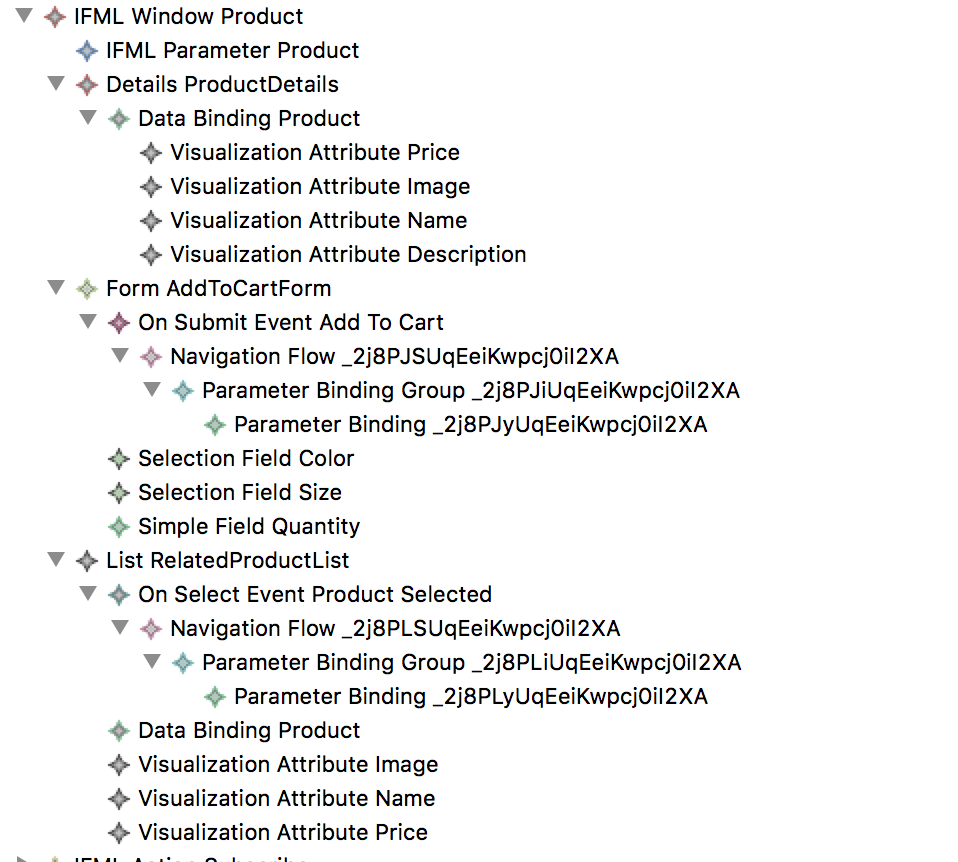
\includegraphics[width=13cm]{images/diagrams/before/ifml-hierarchy-product.png}
  \caption{Interaction Flow Product Model in EMF}
  \label{fig:ifml-before-hierarchy-product}
\end{figure}
\vspace{0.5cm}

\newpage
\subsubsection{Shopping Cart Page}
\label{shopping-cart-page-overview}
The Madison Island Interaction Model for the Shopping Cart page (Figure \ref{fig:desktop-before-shoppingcart} and \ref{fig:ifml-before-shoppingcart}) is  built with a single \textit{IFMLWindow} container with a true-ish \textit{isLandmark} property (flagging the window as accessible from everywhere) including multiple \textit{Form View Component} instances representing the sidebar interactions with the discount codes and shipping estimation widgets. Besides the sidebar, the area holding the cart status and the items in the cart information is displayed with an additional \textit{Form View Component} controlled by the \textit{Activation Condition} responsible for showing items only when the cart is not empty. The section is modelled with a \textit{Form View Component} because of the Qty \textit{SimpleInput} text fields, which allow the user to update the related item quantities or empty the whole cart at any time. Both interactions are controlled with specific \textit{IFMLAction} elements triggered on these \textit{Events}.

\vspace{0.5cm}
\begin{figure}[H]
  \centering
    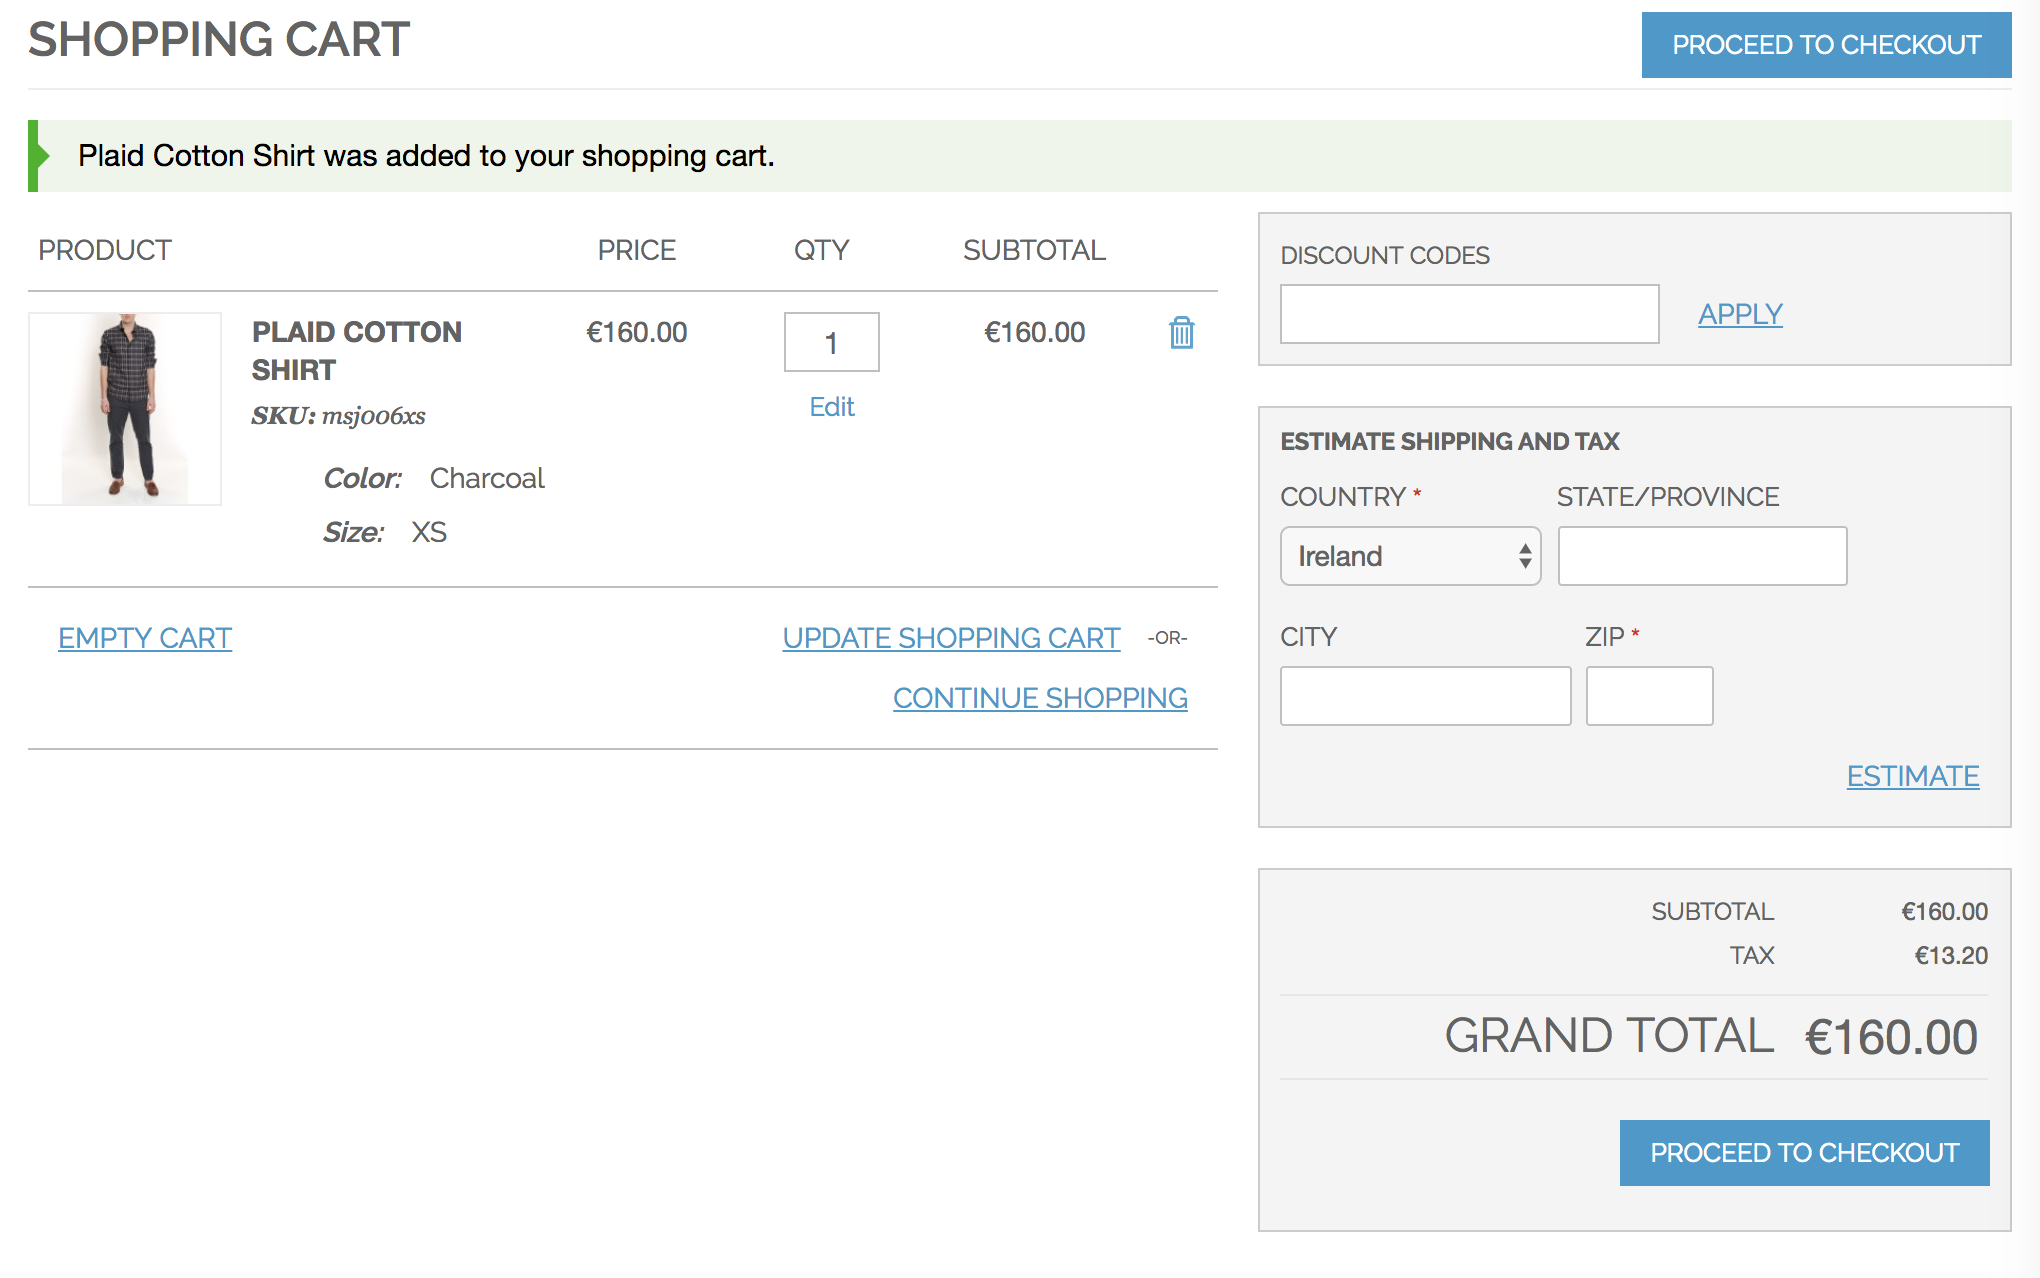
\includegraphics[width=14cm]{images/diagrams/before/desktop-shoppingcart.png}
  \caption{Shopping Cart Page Desktop Version}
  \label{fig:desktop-before-shoppingcart}
\end{figure}

\begin{figure}[H]
  \centering
    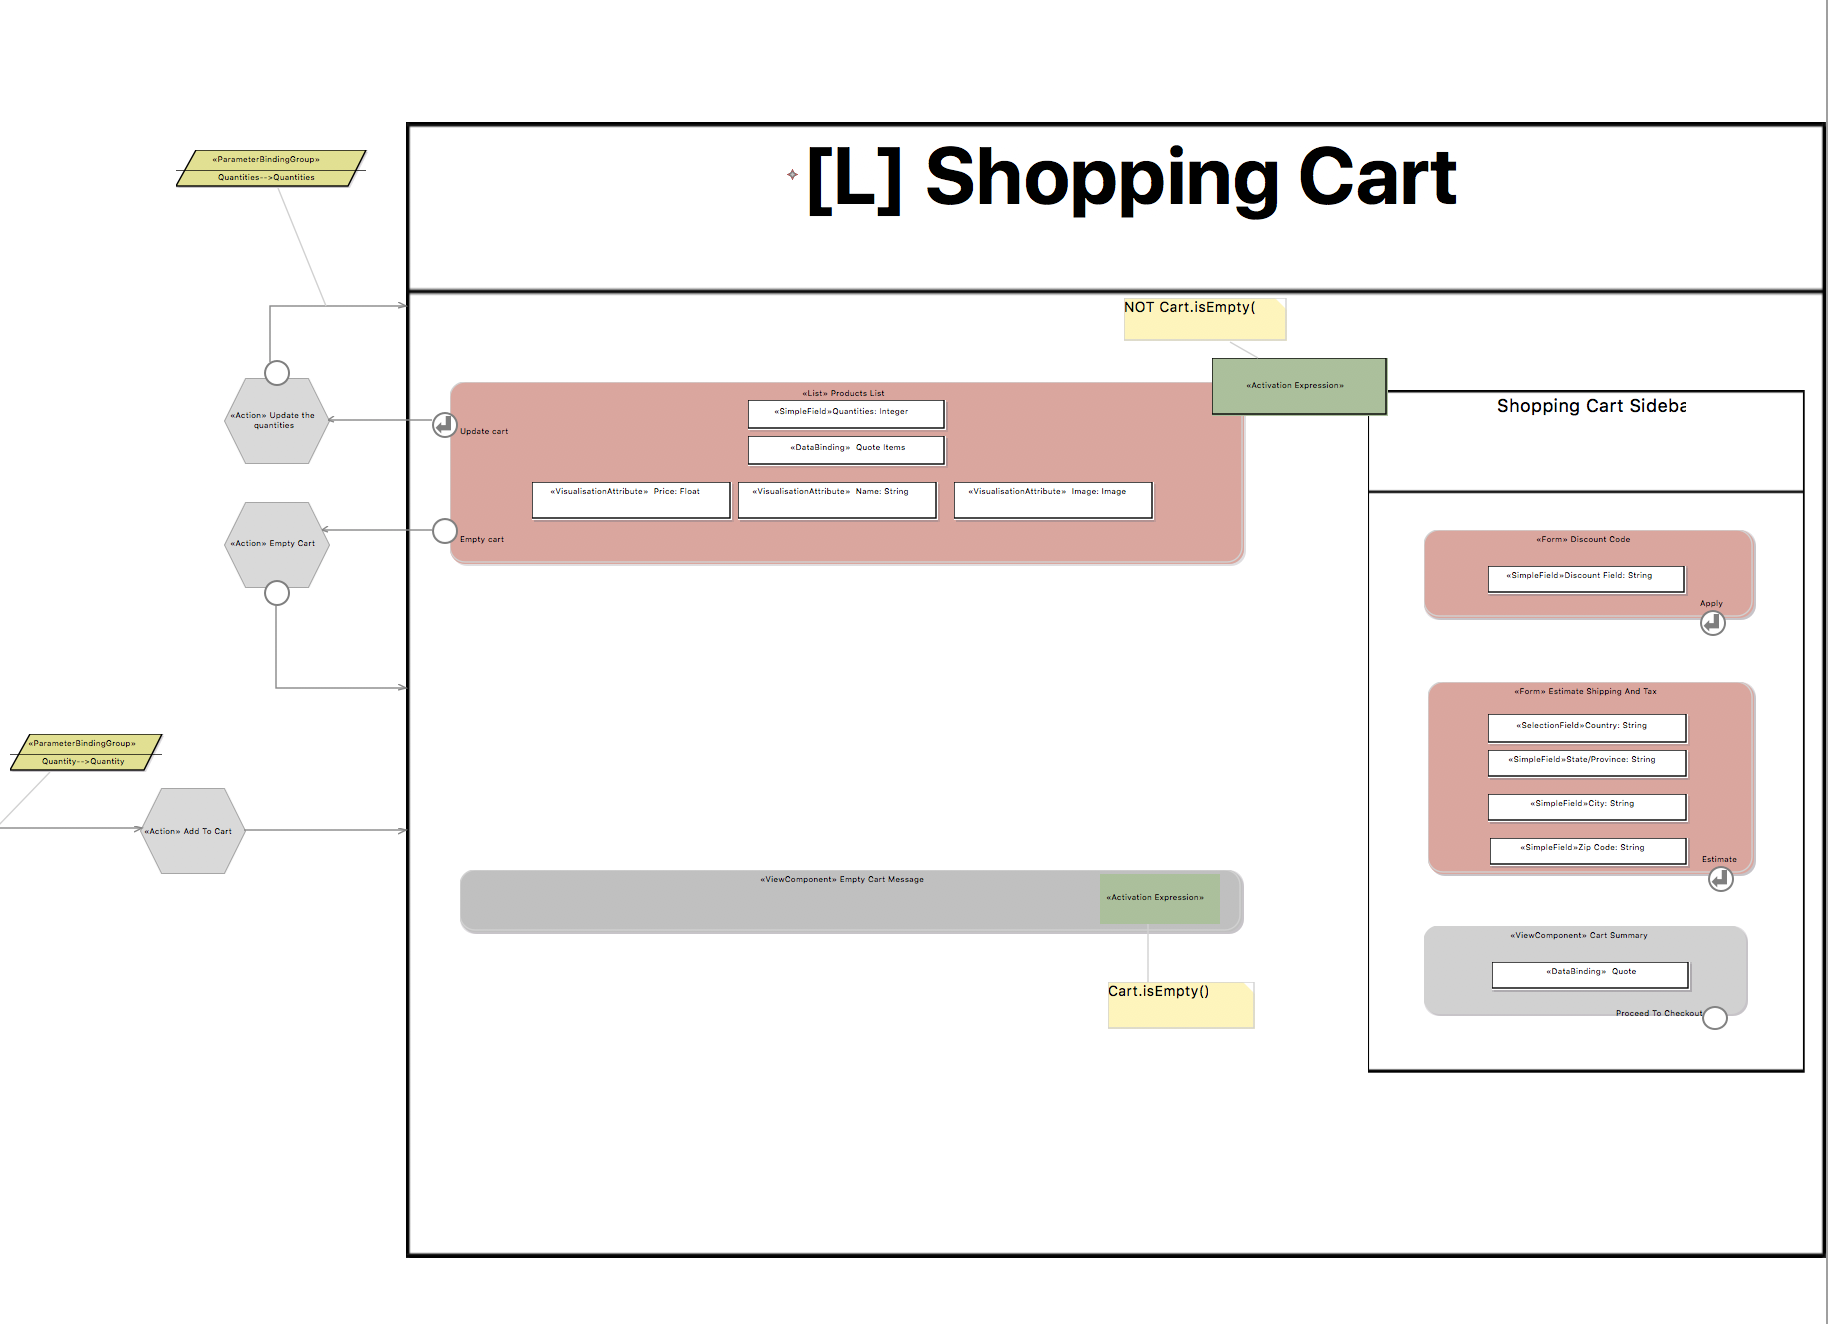
\includegraphics[width=14cm]{images/diagrams/before/ifml-shoppingcart.png}
  \caption{Shopping Cart Page IFML Diagram}
  \label{fig:ifml-before-shoppingcart}
\end{figure}

As shown in Figure \ref{fig:ifml-before-hierarchy-shoppingcart}, the Interaction Flow model representing the shopping page has the following form:
\vspace{0.5cm}
\lstset{language=XML}
\begin{lstlisting} 
    <interactionFlowModelElements xsi:type="ext:IFMLWindow"  name="Product" inInteractionFlows="//@interactionFlowModel/@interactionFlowModelElements.1/@viewElements.2/@viewElementEvents.0/@outInteractionFlows.0 //@interactionFlowModel/@interactionFlowModelElements.0/@viewElements.2/@viewElementEvents.0/@outInteractionFlows.0 //@interactionFlowModel/@interactionFlowModelElements.10/@viewElements.0/@viewElementEvents.0/@outInteractionFlows.0 //@interactionFlowModel/@interactionFlowModelElements.6/@viewElements.1/@viewElements.0/@viewElementEvents.0/@outInteractionFlows.0">
      <parameters  name="Product"/>
      <viewElements xsi:type="ext:Details"  name="ProductDetails">
        <viewComponentParts xsi:type="core:DataBinding"  name="Product" uniformResourceIdentifier="">
          <subViewComponentParts xsi:type="core:VisualizationAttribute"  name="Price" featureConcept="//@domainModel/@domainElements.9"/>
          <subViewComponentParts xsi:type="core:VisualizationAttribute"  name="Image" featureConcept="//@domainModel/@domainElements.7"/>
          <subViewComponentParts xsi:type="core:VisualizationAttribute"  name="Name" featureConcept="//@domainModel/@domainElements.8"/>
          <subViewComponentParts xsi:type="core:VisualizationAttribute"  name="Description" featureConcept="//@domainModel/@domainElements.10"/>
        </viewComponentParts>
      </viewElements>
      <viewElements xsi:type="ext:Form"  name="AddToCartForm">
        <viewElementEvents xsi:type="ext:OnSubmitEvent"  name="Add To Cart" viewElement="//@interactionFlowModel/@interactionFlowModelElements.1/@viewElements.1">
          <outInteractionFlows xsi:type="core:NavigationFlow"  targetInteractionFlowElement="//@interactionFlowModel/@interactionFlowModelElements.9">
            <parameterBindingGroup >
              <parameterBindings  sourceParameter="//@interactionFlowModel/@interactionFlowModelElements.1/@viewElements.1/@viewComponentParts.2" targetParameter="//@interactionFlowModel/@interactionFlowModelElements.1/@viewElements.1/@viewComponentParts.2"/>
            </parameterBindingGroup>
          </outInteractionFlows>
        </viewElementEvents>
        <viewComponentParts xsi:type="ext:SelectionField"  name="Color" />
        <viewComponentParts xsi:type="ext:SelectionField"  name="Size" />
        <viewComponentParts xsi:type="ext:SimpleField"  name="Quantity" />
      </viewElements>
      <viewElements xsi:type="ext:List"  name="RelatedProductList">
        <viewElementEvents xsi:type="ext:OnSelectEvent"  name="Product Selected" viewElement="//@interactionFlowModel/@interactionFlowModelElements.1/@viewElements.2">
          <outInteractionFlows xsi:type="core:NavigationFlow"  targetInteractionFlowElement="//@interactionFlowModel/@interactionFlowModelElements.1">
            <parameterBindingGroup >
              <parameterBindings  sourceParameter="//@interactionFlowModel/@interactionFlowModelElements.0/@viewElements.2/@parameters.0" targetParameter="//@interactionFlowModel/@interactionFlowModelElements.1/@parameters.0"/>
            </parameterBindingGroup>
          </outInteractionFlows>
        </viewElementEvents>
        <viewComponentParts xsi:type="core:DataBinding"  name="Product"/>
        <viewComponentParts xsi:type="core:VisualizationAttribute"  name="Image" featureConcept="//@domainModel/@domainElements.7"/>
        <viewComponentParts xsi:type="core:VisualizationAttribute"  name="Name" featureConcept="//@domainModel/@domainElements.8"/>
        <viewComponentParts xsi:type="core:VisualizationAttribute"  name="Price" featureConcept="//@domainModel/@domainElements.9"/>
      </viewElements>
    </interactionFlowModelElements>
\end{lstlisting}

The \textit{IFMLModel} representation of the Shopping Cart page structure is presented in Figure~\ref{fig:ifml-before-hierarchy-shoppingcart}

\vspace{0.5cm}
\begin{figure}[H]
  \centering
    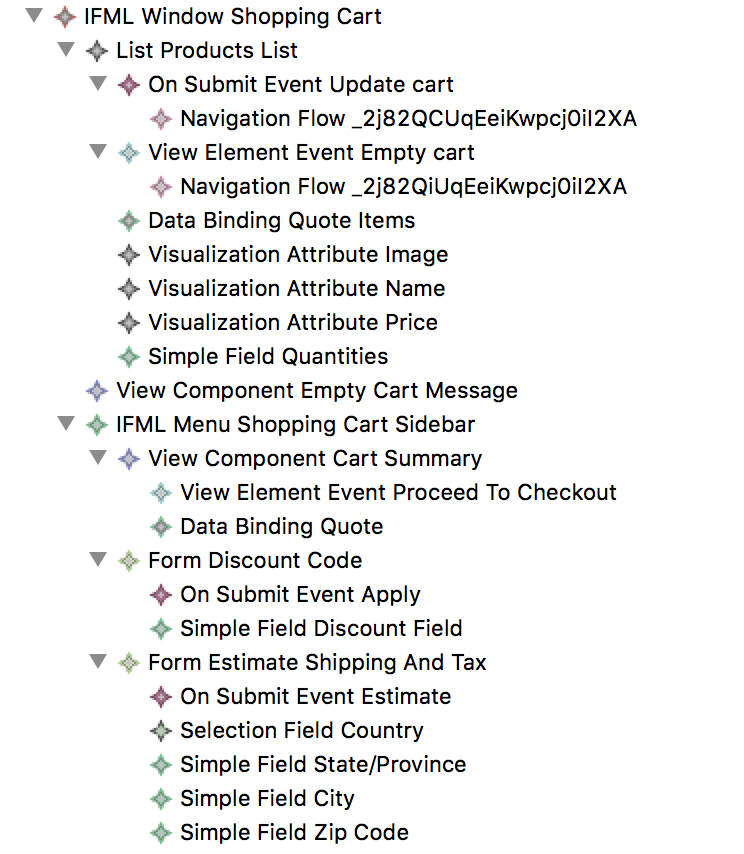
\includegraphics[width=12cm]{images/diagrams/before/ifml-hierarchy-shoppingcart.png}
  \caption{Interaction Flow Shopping Cart Model in EMF}
  \label{fig:ifml-before-hierarchy-shoppingcart}
\end{figure}
\vspace{0.5cm}

\subsubsection{Shared Elements and Interactions}

As mentioned previously, shared sections of the platform such as the Header and the Footer have been modelled as \textit{IFMLWindow} nodes reachable from any other area of the website, thus their \textit{isLandmark} attribute set to true. In more detail, the Header section contains a Navigation Menu in the form of a \textit{List View Component} with a children \textit{DataBinding} component correlated to the Category \textit{Domain Model} and a simple \textit{Form View Component} for the search mechanism. When the user performs a search submitting a keyword, the \textit{SearchKeyword} is triggered and the Search Keyword \textit{IFMLAction} is executed based on the parameters held in the associated \textit{ParameterBinding} element.  The resulting Search Results page, which presents a sidebar for filtering and a list of items matching the search, is another \textit{IFMLWindow}, whose structure resembles the ``Product List Mode" for a Category Page described earlier (Figure \ref{fig:ifml-before-header-search}).

\vspace{0.5cm}
\begin{figure}[H]
  \centering
    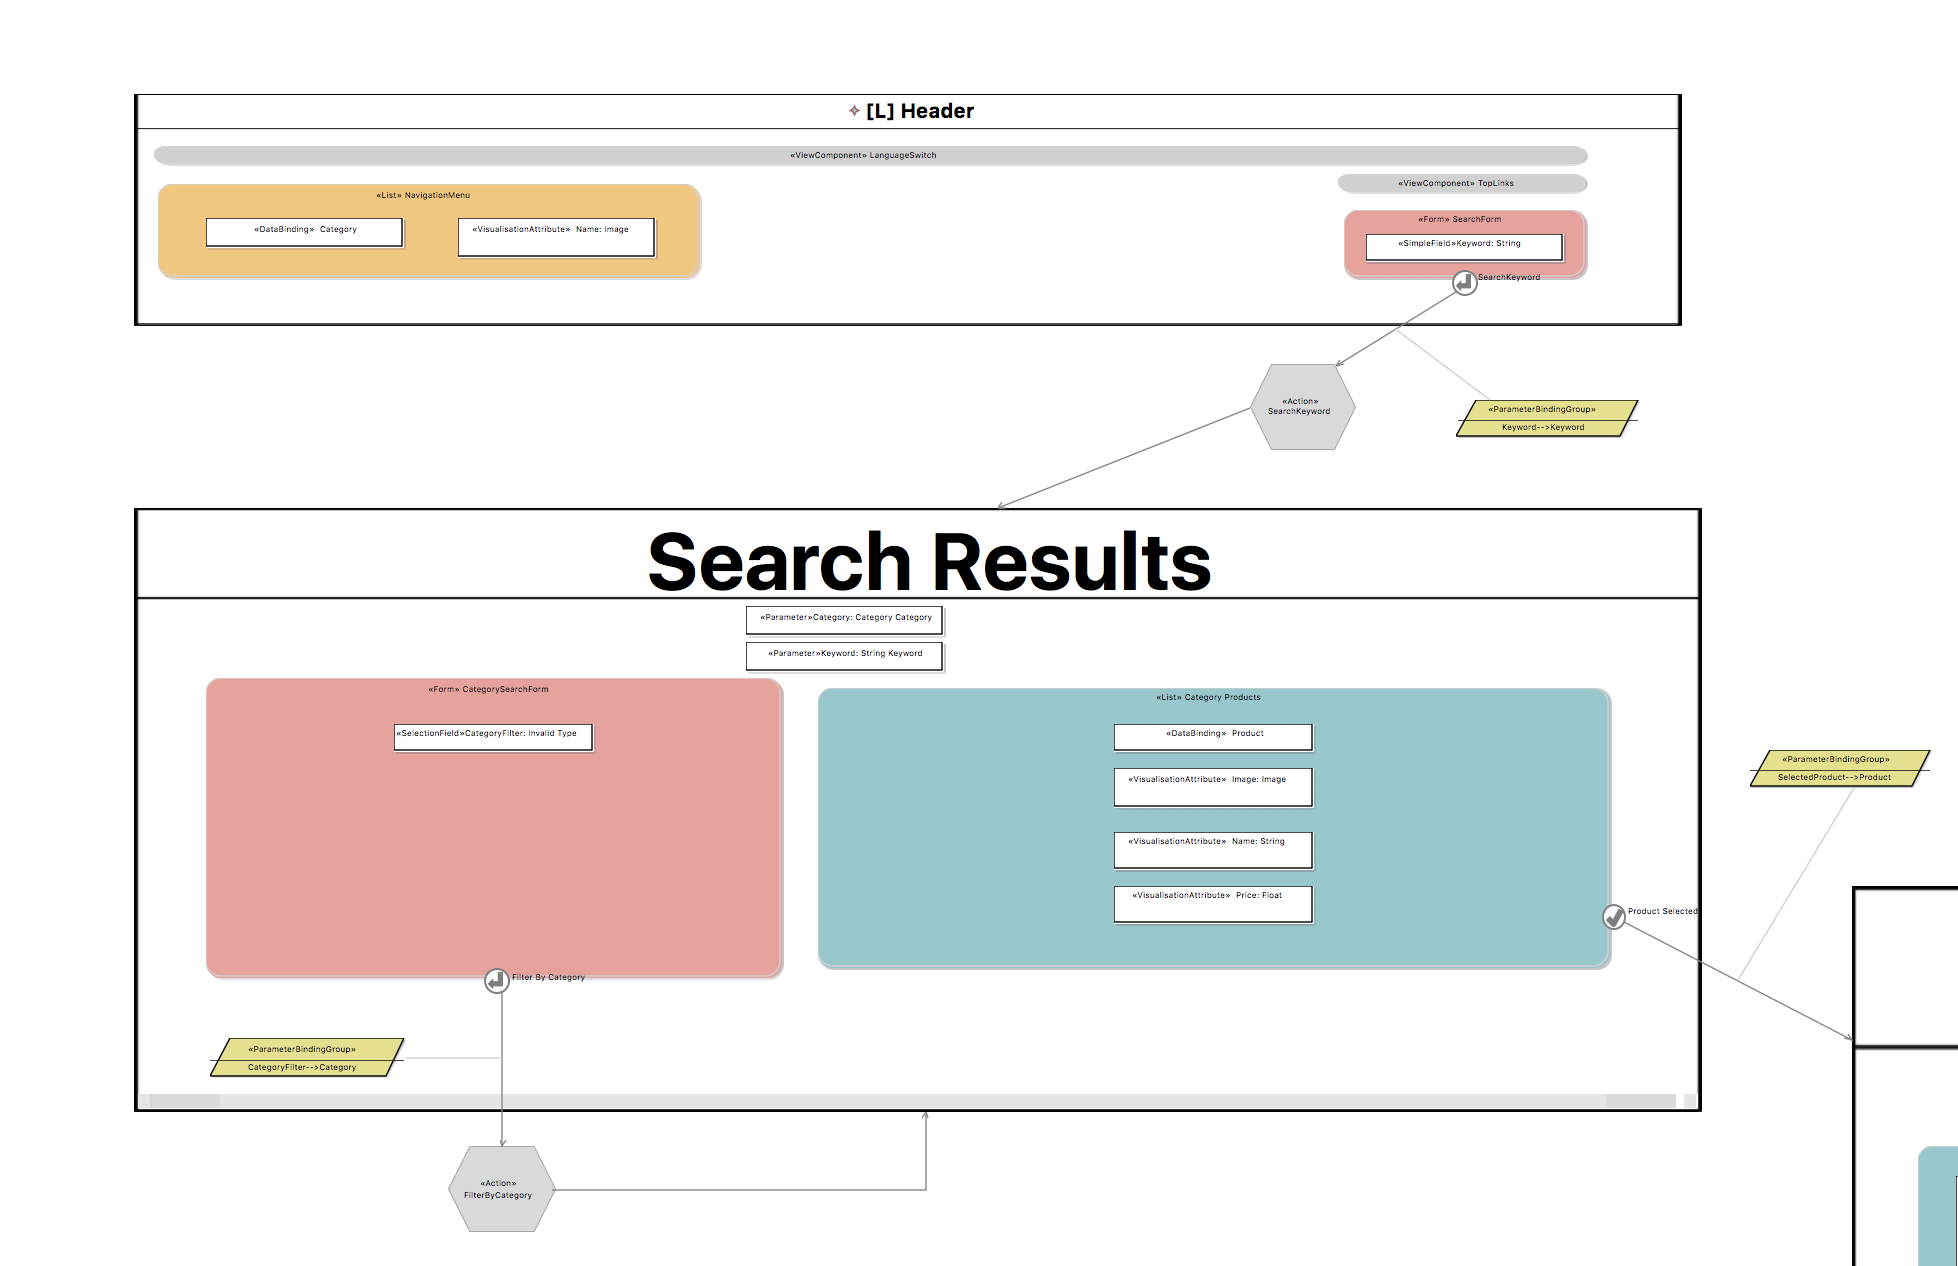
\includegraphics[width=12cm]{images/diagrams/before/ifml-header-search.png}
  \caption{Header and Search sections IFML Diagrams}
  \label{fig:ifml-before-header-search}
\end{figure}
\vspace{0.5cm}

The Footer \textit{IFMLWindow} model is quite straightforward. It retains the information about the footer links presented on the bottom of all the pages of the website in the form of a simple \textit{ViewComponent} and a Newsletter subscription \textit{Form View Component} reacting to SubscribeNewsletter submit \textit{Events}. Similarly to the header case we have just described, the email passed as an argument from the \textit{Event} is carried to the \textit{IFMLAction} which, in this specific case, performs the actual Customer subscription and redirects them to the current page.(Figure \ref{fig:ifml-before-footer}).

\vspace{0.5cm}
\begin{figure}[H]
  \centering
    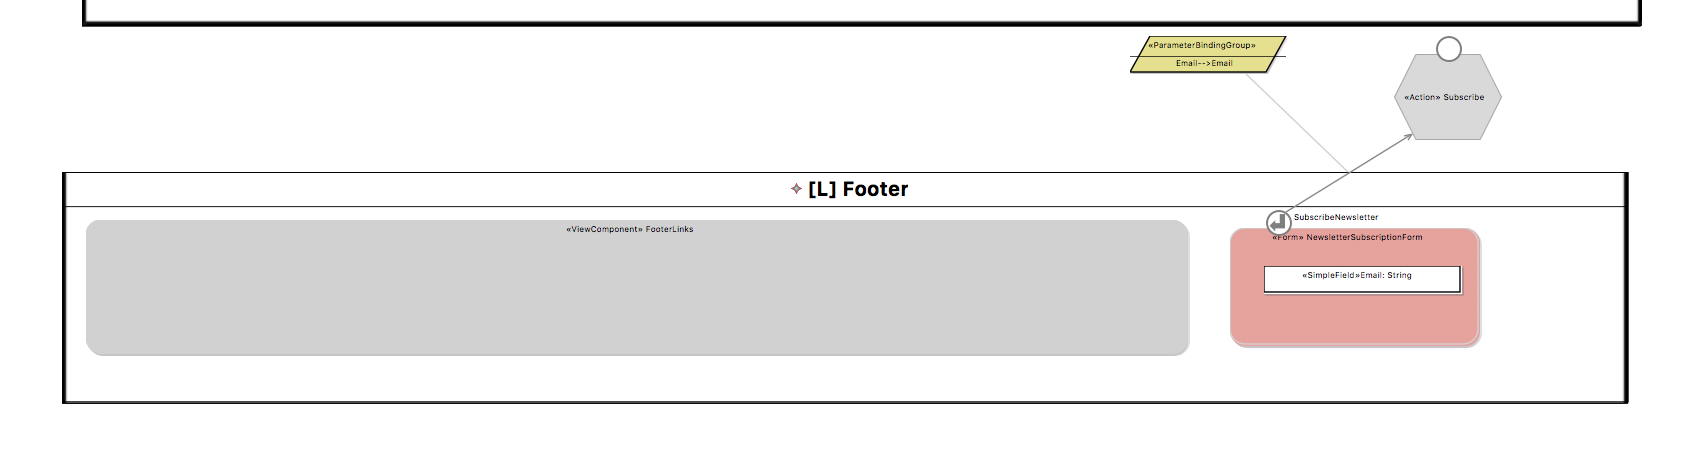
\includegraphics[width=12cm]{images/diagrams/before/ifml-footer.png}
  \caption{Footer section IFML Diagram}
  \label{fig:ifml-before-footer}
\end{figure}
\vspace{0.5cm}

\newpage
We conclude this chapter with both a snippet of the Header \textit{IFMLWindow} element code coming from the \textit{IFMLModel}, and an excerpt of the ecore model diagram in EMF for the areas of the website we described in this subsection (Figure \ref{fig:ifml-before-hierarchy-headersearchfooter}).

\vspace{0.5cm}
\lstset{language=XML}
\begin{lstlisting} 
  <interactionFlowModelElements xsi:type="ext:IFMLWindow" id="_LvuL0BPREei3TrqMA9Bdvw" name="Header" isLandmark="true">
  <viewElements xsi:type="ext:List" id="_v0p5YA9BEeiZ14TmPBeBNA" name="NavigationMenu">
    <viewComponentParts xsi:type="core:DataBinding" id="__mcXIA9BEeiZ14TmPBeBNA" name="Category"/>
    <viewComponentParts xsi:type="core:VisualizationAttribute" id="_Kbzt3xIZEeijSslFDgCgZA" name="Name" featureConcept="//@domainModel/@domainElements.5"/>
  </viewElements>
  <viewElements xsi:type="ext:Form" id="_YWvrMA9GEeiZ14TmPBeBNA" name="SearchForm">
    <viewElementEvents xsi:type="ext:OnSubmitEvent" id="_ULm7WRIWEeijSslFDgCgZA" name="SearchKeyword" viewElement="//@interactionFlowModel/@interactionFlowModelElements.4/@viewElements.1">
      <outInteractionFlows xsi:type="core:NavigationFlow" id="_Y6uV1xIWEeijSslFDgCgZA" targetInteractionFlowElement="//@interactionFlowModel/@interactionFlowModelElements.3">
        <parameterBindingGroup id="_yCY84hPOEei3TrqMA9Bdvw">
          <parameterBindings id="_y5vbohPOEei3TrqMA9Bdvw" sourceParameter="//@interactionFlowModel/@interactionFlowModelElements.4/@viewElements.1/@viewComponentParts.0" targetParameter="//@interactionFlowModel/@interactionFlowModelElements.3/@parameters.0"/>
        </parameterBindingGroup>
      </outInteractionFlows>
    </viewElementEvents>
    <viewComponentParts xsi:type="ext:SimpleField" id="_lWoCAA9GEeiZ14TmPBeBNA" name="Keyword" direction="out" />
  </viewElements>
  <viewElements xsi:type="core:ViewComponent" id="_aQFfjQ9TEeiZ14TmPBeBNA" name="TopLinks"/>
  <viewElements xsi:type="core:ViewComponent" id="_ezXdfQ9TEeiZ14TmPBeBNA" name="LanguageSwitch"/>
</interactionFlowModelElements>
\end{lstlisting}
\vspace{0.5cm}


\vspace{0.5cm}
\begin{figure}[H]
  \centering
    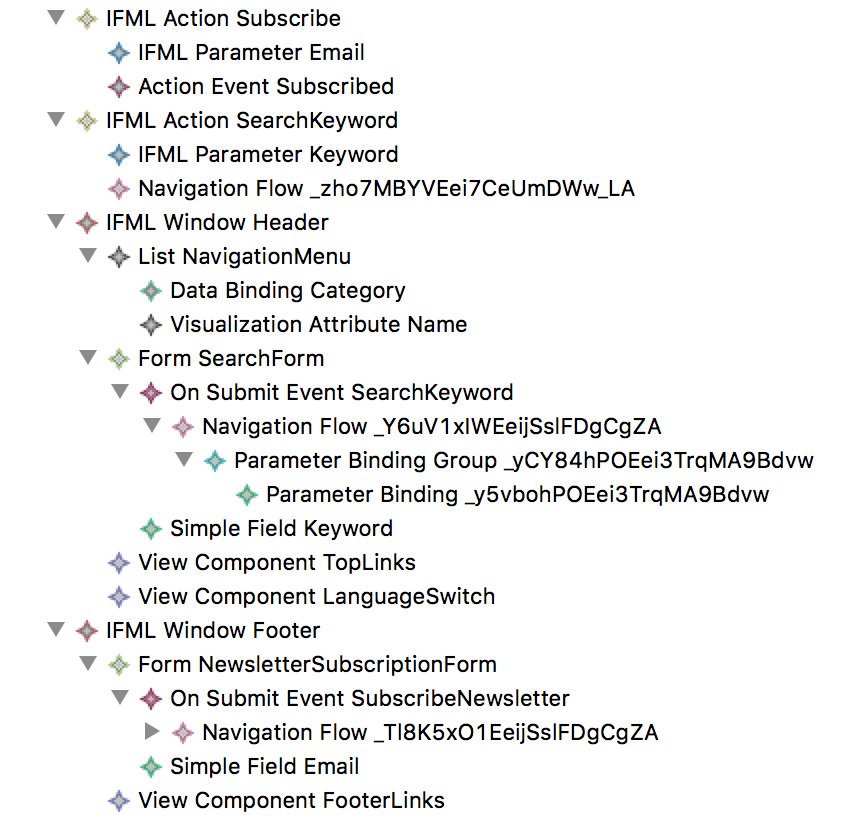
\includegraphics[width=12cm]{images/diagrams/before/ifml-hierarchy-headersearchfooter.png}
  \caption{Interaction Flow for the shared elements in EMF}
  \label{fig:ifml-before-hierarchy-headersearchfooter}
\end{figure}
\vspace{0.5cm}

